% Options for packages loaded elsewhere
\PassOptionsToPackage{unicode}{hyperref}
\PassOptionsToPackage{hyphens}{url}
%
\documentclass[
]{article}
\title{Planning for Urban Satisfaction}
\author{Yuanzhao WANG}
\date{2022-03-22}

\usepackage{amsmath,amssymb}
\usepackage{lmodern}
\usepackage{iftex}
\ifPDFTeX
  \usepackage[T1]{fontenc}
  \usepackage[utf8]{inputenc}
  \usepackage{textcomp} % provide euro and other symbols
\else % if luatex or xetex
  \usepackage{unicode-math}
  \defaultfontfeatures{Scale=MatchLowercase}
  \defaultfontfeatures[\rmfamily]{Ligatures=TeX,Scale=1}
\fi
% Use upquote if available, for straight quotes in verbatim environments
\IfFileExists{upquote.sty}{\usepackage{upquote}}{}
\IfFileExists{microtype.sty}{% use microtype if available
  \usepackage[]{microtype}
  \UseMicrotypeSet[protrusion]{basicmath} % disable protrusion for tt fonts
}{}
\makeatletter
\@ifundefined{KOMAClassName}{% if non-KOMA class
  \IfFileExists{parskip.sty}{%
    \usepackage{parskip}
  }{% else
    \setlength{\parindent}{0pt}
    \setlength{\parskip}{6pt plus 2pt minus 1pt}}
}{% if KOMA class
  \KOMAoptions{parskip=half}}
\makeatother
\usepackage{xcolor}
\IfFileExists{xurl.sty}{\usepackage{xurl}}{} % add URL line breaks if available
\IfFileExists{bookmark.sty}{\usepackage{bookmark}}{\usepackage{hyperref}}
\hypersetup{
  pdftitle={Planning for Urban Satisfaction},
  pdfauthor={Yuanzhao WANG},
  hidelinks,
  pdfcreator={LaTeX via pandoc}}
\urlstyle{same} % disable monospaced font for URLs
\usepackage[margin=1in]{geometry}
\usepackage{graphicx}
\makeatletter
\def\maxwidth{\ifdim\Gin@nat@width>\linewidth\linewidth\else\Gin@nat@width\fi}
\def\maxheight{\ifdim\Gin@nat@height>\textheight\textheight\else\Gin@nat@height\fi}
\makeatother
% Scale images if necessary, so that they will not overflow the page
% margins by default, and it is still possible to overwrite the defaults
% using explicit options in \includegraphics[width, height, ...]{}
\setkeys{Gin}{width=\maxwidth,height=\maxheight,keepaspectratio}
% Set default figure placement to htbp
\makeatletter
\def\fps@figure{htbp}
\makeatother
\setlength{\emergencystretch}{3em} % prevent overfull lines
\providecommand{\tightlist}{%
  \setlength{\itemsep}{0pt}\setlength{\parskip}{0pt}}
\setcounter{secnumdepth}{-\maxdimen} % remove section numbering
\ifLuaTeX
  \usepackage{selnolig}  % disable illegal ligatures
\fi

\begin{document}
\maketitle

--A critical approach to measure the quality of urban experience from a
social media platform Yuanzhao WANG THESIS RESEARCH MDES ULE 2022
Supervisor: Prof.~Carole Voulgaris

\hypertarget{abstract}{%
\section{Abstract}\label{abstract}}

This paper aims to examine the strengths and weaknesses of social media
platforms and proposes a vision for a better platform to invite
bottom-up citizen participation in data-driven urban planning for urban
satisfaction. The research proposes a method to measure the emotional
response of individual citizens to the characteristics of the built
environment focusing on proximity and convenience between pedestrians
and nearby commercial and cultural activities. The goal is to explore
the relationships between citizens' sentiments, urban form, and urban
activities, and build a regression model for optimizing urban
satisfaction. By examining the existing Weibo data, the initial research
revealed serious limitations that existing social media data that would
merely provide sufficient information for quantitative urban planning.
Finally, it proposes a better platform that can fulfill the need for
more accurate data for quantifying individual urban satisfaction.

\hypertarget{introduction}{%
\section{Introduction}\label{introduction}}

In China, the early stage of urbanization was subject to the national
ambition and development, whose aim at boosting the economic production
and consumption. As such, hundreds and thousands of cities and towns
were built to serve for this purpose that plays an important role in
improving the national economy based on the scarification of natural
resource and incline of factory production (Zhang et al., 2020).
However, since the decreasing demand for industrial production and the
arise of urban awareness of residents happiness, the government has
issued the ``New Urbanization (citization and townization) Policy'' and
``Specialty Townization Policy'' since 2014, increasingly focus on
citizen wellbeing, urban governance and the urban environment (State
Council of China, 2014).

The new urban policies in China shifted the emphasis of urbanization
away from economic development and toward human-centric development,
improving residents' wellbeing and building new ecological smart cities.
However, the evaluation of residents' wellbeing and urban planning
process remains top-down and entirely conducted by governments and
experts (figure 1). The qualitative surveys and reports could only cover
a small proportion of population, and it becomes even harder and
time-consuming as the population in cities and towns reached 848
millions (State Council of China, 2010).

\href{https://WTHSYZW.github.io/Thesis_2022/maps/topdown.pdf}{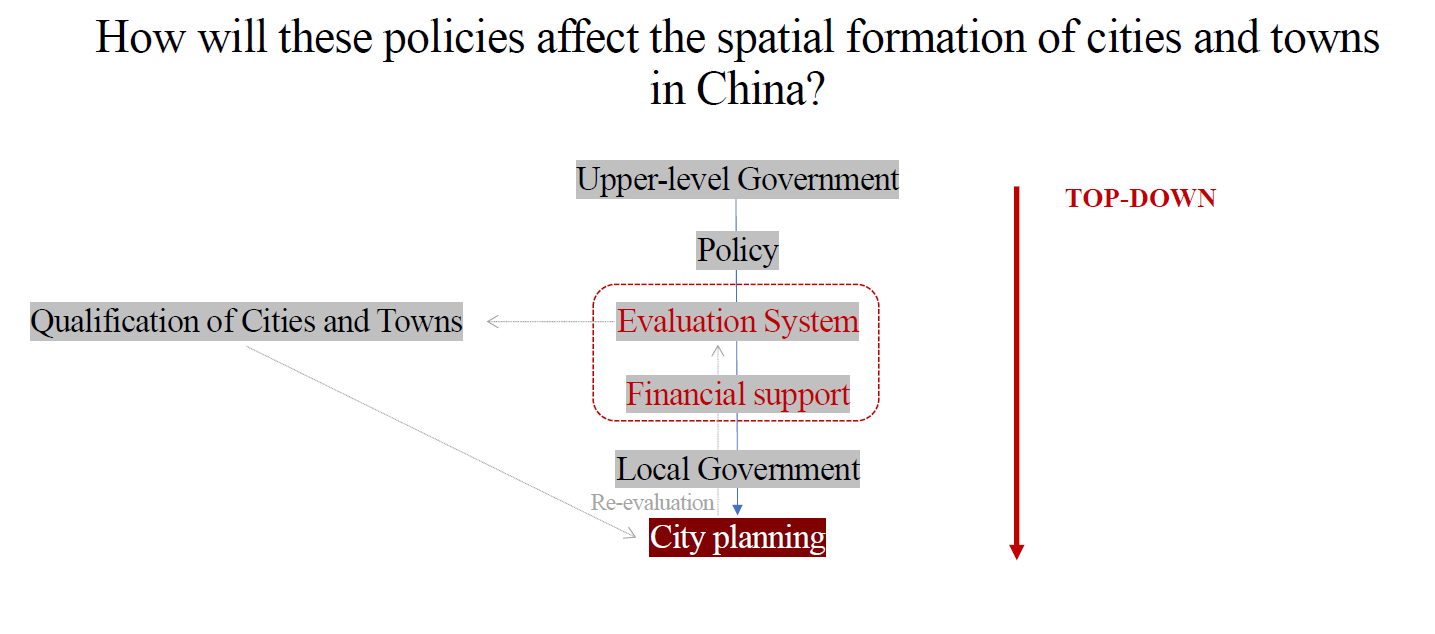
\includegraphics{maps/topdown.png}}\\
figure 1 Top-down urban planning in China

With the introduction of social media data and machine learning
technologies, new bottom-up data and methods for studying urban spatial
patterns and residents' life have emerged. The ideal bottom-up data for
planner should have three characteristics. First, easy Participation:
People should be easy to participate, which means people don't need to
leave a period of time and show up in a specific place to engage.
Second, public Access: most people should be able to access. Lastly,
people should be able to express their long-tome expectations of the
city and their satisfaction regarding the existing conditions.

In 2022, there were more than 1.02 billion people have access to mobile
internet, while 68\% of them frequently use social media platform
(DataReportal, 2022). The large population coverage and easy
participation of social media data can meet some of the needs of ideal
data, but not all of them. Existing data can only generate real-time
daily experiences that are not specific to the built environment or
long-term well-being (figure 2).

\href{https://WTHSYZW.github.io/Thesis_2022/maps/comparison.png}{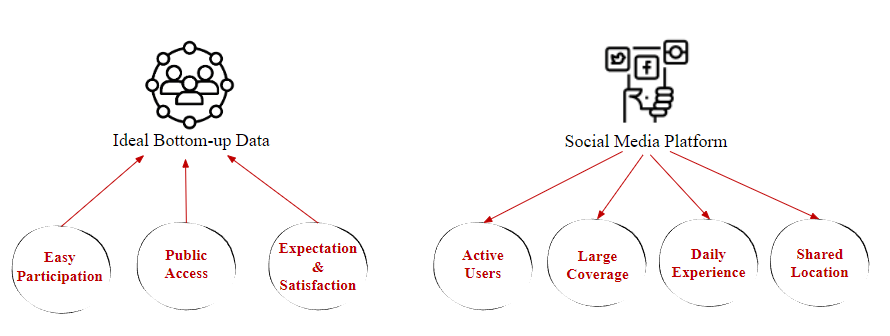
\includegraphics{maps/comparison.png}}
figure 2 comparison between ideal data and existing social media data

To address the shortcomings of existing data and break the traditional
top-down approach to urban planning, a thorough validation and a
quantitative framework is required. I propose a research framework
measuring the emotional response of individual citizens to the
characteristics of the built environment focusing on proximity and
convenience between pedestrians and nearby commercial and cultural
activities. The goal is to explore the relationships between citizens'
satisfaction, urban form, and urban activities. This approach can be
applied to bring public satisfaction into the urban planning process
through the social platform as a way to quantify the quality of urban
life (figure 2). However, the simulation model based on the existing
Weibo data revealed serious limitations. The discussion of the strengths
and drawbacks of existing social media data leads to a vision for a
better platform to invite bottom-up citizen participation in data-driven
urban planning for urban satisfaction.

\href{https://WTHSYZW.github.io/Thesis_2022/maps/proposaldiagram.png}{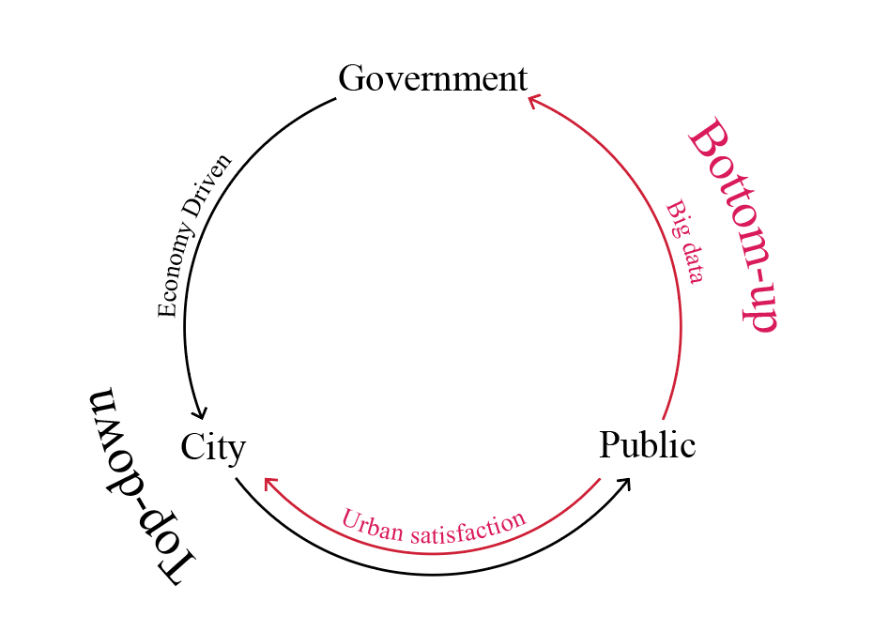
\includegraphics{maps/proposaldiagram.png}}
figure 3 Proposal diagram

\hypertarget{literature-review}{%
\section{Literature Review}\label{literature-review}}

\hypertarget{wellbeing-as-a-measure-of-health-and-the-built-environment}{%
\subsection{Wellbeing as a Measure of Health and the Built
environment}\label{wellbeing-as-a-measure-of-health-and-the-built-environment}}

Scientists have historically measured well-being using objective
indicators (e.g., GDP, health, employment, literacy, poverty) and
increasing measured subjective well-being that influences individual
life. Modern measures of well-being that account for cognitive
evaluations (i.e., evaluative well-being) and reactions to experiences
(i.e., experienced well-being) have therefore become the ``currency of a
life that matters'' (Rath et al., 2010). As the concept of well-being
develops, the indices including physical health, mental health, air
quality and more are increasingly used, implying a strong relationship
between health and residents' well-being (Diener et al., 1999; Lawless
\& Lucas, 2010). Mouratidis (2018) further investigated different
aspects of subjective well-being (SWB): hedonic, life satisfaction, and
eudaimonic. He categorized neighborhood characteristics into objective
and perceived, and proposed a conceptual framework to explain how
neighborhood characteristics might affect SWB by inviting a mediating
factors such as personal relationships, leisure activities, health, and
neighborhood impact on emotions and mood.There are increasing numbers of
studies investigating how the built environment may affect individual
wellbeing. Some studies found that population density may affect
well-being on the city level (Florida et al., 2013). Social and human
capital, considered significant drivers of urban well-being, can be
affected by safety, educational opportunities, and access to arts and
culture (Leyden et al., 2011; Florida et al., 2013). Other aspects of
urban infrastructure (such as roads and transportation) impact commute
time and connectedness, both of which are related to happiness (Yin et
al., 2021; Gim, 2021).

\hypertarget{big-data-social-media-and-sentiment-analysis}{%
\subsection{Big data, Social media and Sentiment
analysis}\label{big-data-social-media-and-sentiment-analysis}}

Recently, the availability of mobile information, big urban data and
machine learning technology has significantly enhanced urban research
methods, particularly in terms of the dynamic spatial and temporal
relationships between human behavior and urban research (Wu, Ye, Ren, \&
Du, 2018). The invitation of various big data could change China's
top-down urban planning process by bringing individual information into
the discussion of urban space and quality. With the rise of social media
and machine learning, sentiment analysis became a field of study that
mines public opinions, measures subjective happiness and relates them to
different research areas. The previous studies applied Twitter, Sina
Weibo data (Chinese Twitter) and Dazhong dianping (Chinese Yelp) to
examine the relationship between urban form, spatial quality, and public
comments, such as the relationship between quality of urban parks and
travelers' behavior and words; urban transportation and commercial
facilities (Li et al., 2018; Ta et al., 2020; Yao et al., 2019; Plunz et
al., 2019). Some research further studied the difference and
distribution of residents' emotions regarding gender, time-dimension and
different urban facilities (Ma et al., 2020; Zhen et al., 2018).

\hypertarget{quantitative-urban-measure-of-the-built-environment}{%
\subsection{Quantitative urban measure of the built
environment}\label{quantitative-urban-measure-of-the-built-environment}}

The measurement of the built environment is constructed by a variety
body of indices to address different urban issues. Cervero and
Kockelman's developed initial ``three Ds'' (density, design, and
diversity) in 1997 to evaluate the existing urban built environment.
Edwing et al.~expanded on this concept by adding two Ds (destination
accessibility and transportation distance) (Ewing \& Cervero, 2001;
Ewing et al., 2009). More Ds were added afterwards to reflect the
changing built environment, such as Demand management and Demographics
(Ewing \& Cervero, 2010). Scholars have modified the list of variables
based on these quantitative frameworks to comprehensively examine the
built environment while addressing various urban issues and topics. Some
research used relative entropy to discern compactness from sprawl in the
built environment (Tsai, 2005). Others used a multi-metric urban
intensity index at a metropolitan scale, which included land use,
infrastructure, and landscape variables in addition to density and
compactness (Tate et al., 2005). More recent studies, especially in the
Chinese context, Rowe et al.~(2014) proposed the measurement of urban
intensity from variables of compactness, density, diversity, and
connectivity, aiming at revealing the resource distribution,
transportation efficiency, and social integration in both cities and
optimize the urban performance (Rowe et al., 2014). Later, Guan and Rowe
(2016) evaluated the spatial structure of small towns in Zhejiang
Province using similar urban intensity characteristics, such as density,
compactness, diversity, and accessibility.

\hypertarget{research-questions}{%
\subsection{Research questions}\label{research-questions}}

In this research, my thesis mainly discussed three research questions:

\begin{itemize}
\tightlist
\item
  What kind of data is needed for urban planner? And how to build a
  method framework to optimize satisfaction \& wellbeing?\\
\item
  If existing social media data is not enough, what are the
  shortcomings?\\
\item
  What better data-gathering tool might be better than existing social
  media platforms?
\end{itemize}

\hypertarget{methodology}{%
\section{Methodology}\label{methodology}}

The research aims to apply sentiment analysis to quantify qualitative
public sentiment from text-based information as a representation of
urban satisfaction, and develop multivariate regression models to
explore the relationship between urban satisfaction from social media
and the built environment in China. Based on the models, this research
compare existing condition and the planned condition of Jiaxing city in
China, and test different planning scenarios to explore the possible
changes of urban satisfaction when using existing data from social media
platform (figure 4).

\href{https://WTHSYZW.github.io/Thesis_2022/maps/workflow.png}{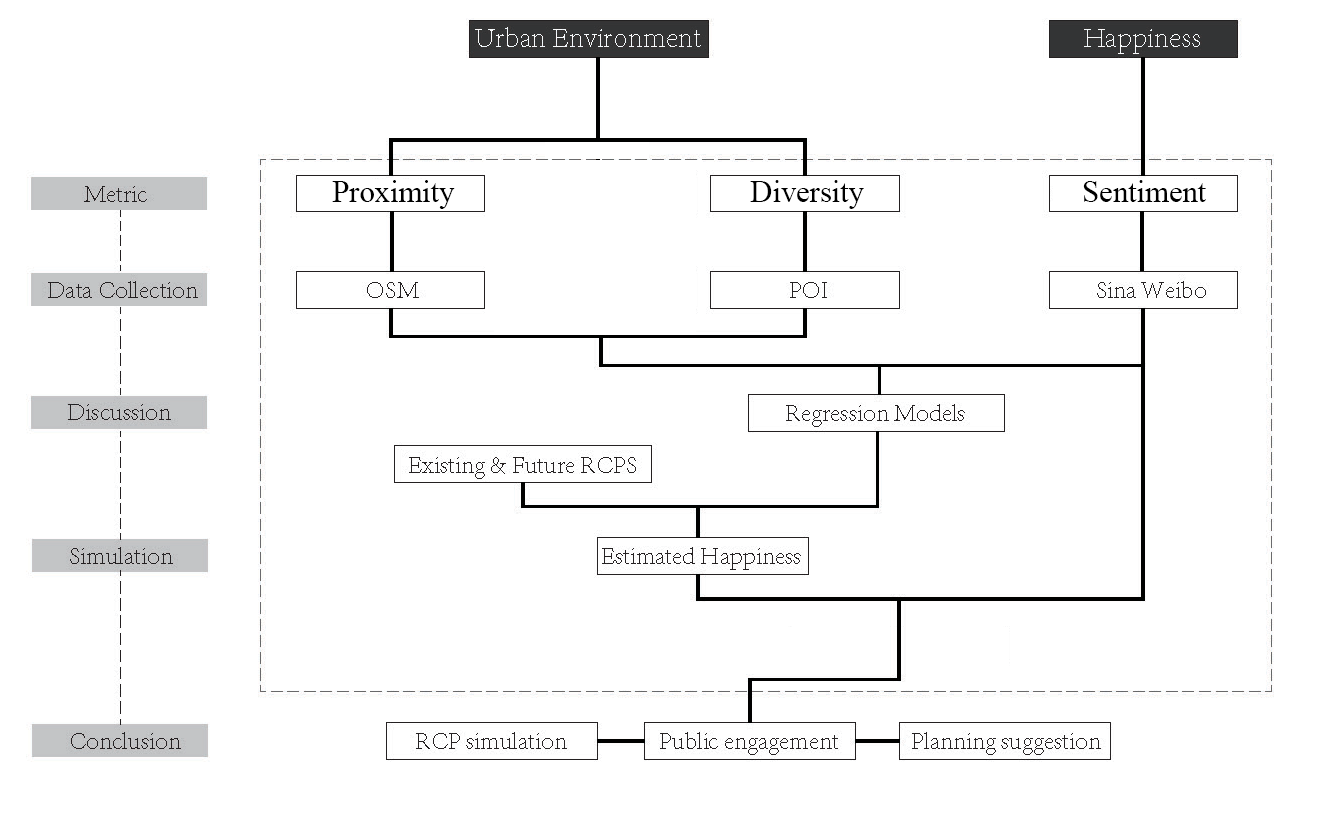
\includegraphics{maps/workflow.png}}
figure 4 Research framework

\hypertarget{site}{%
\subsection{Site}\label{site}}

The study area is Jiaxing city in China's Zhejiang province (figure 5).
Jiaxing is a significant city that is part of the Yangtze River Delta
city cluster and the Shanghai metropolitan area. It is located in close
proximity to the two major cities of Shanghai and Hangzhou. It is a
small tourist city with two counties, 44 towns, and 809 administrative
villages that has been designated as a national key program.

\href{https://WTHSYZW.github.io/Thesis_2022/maps/jiaxing.png}{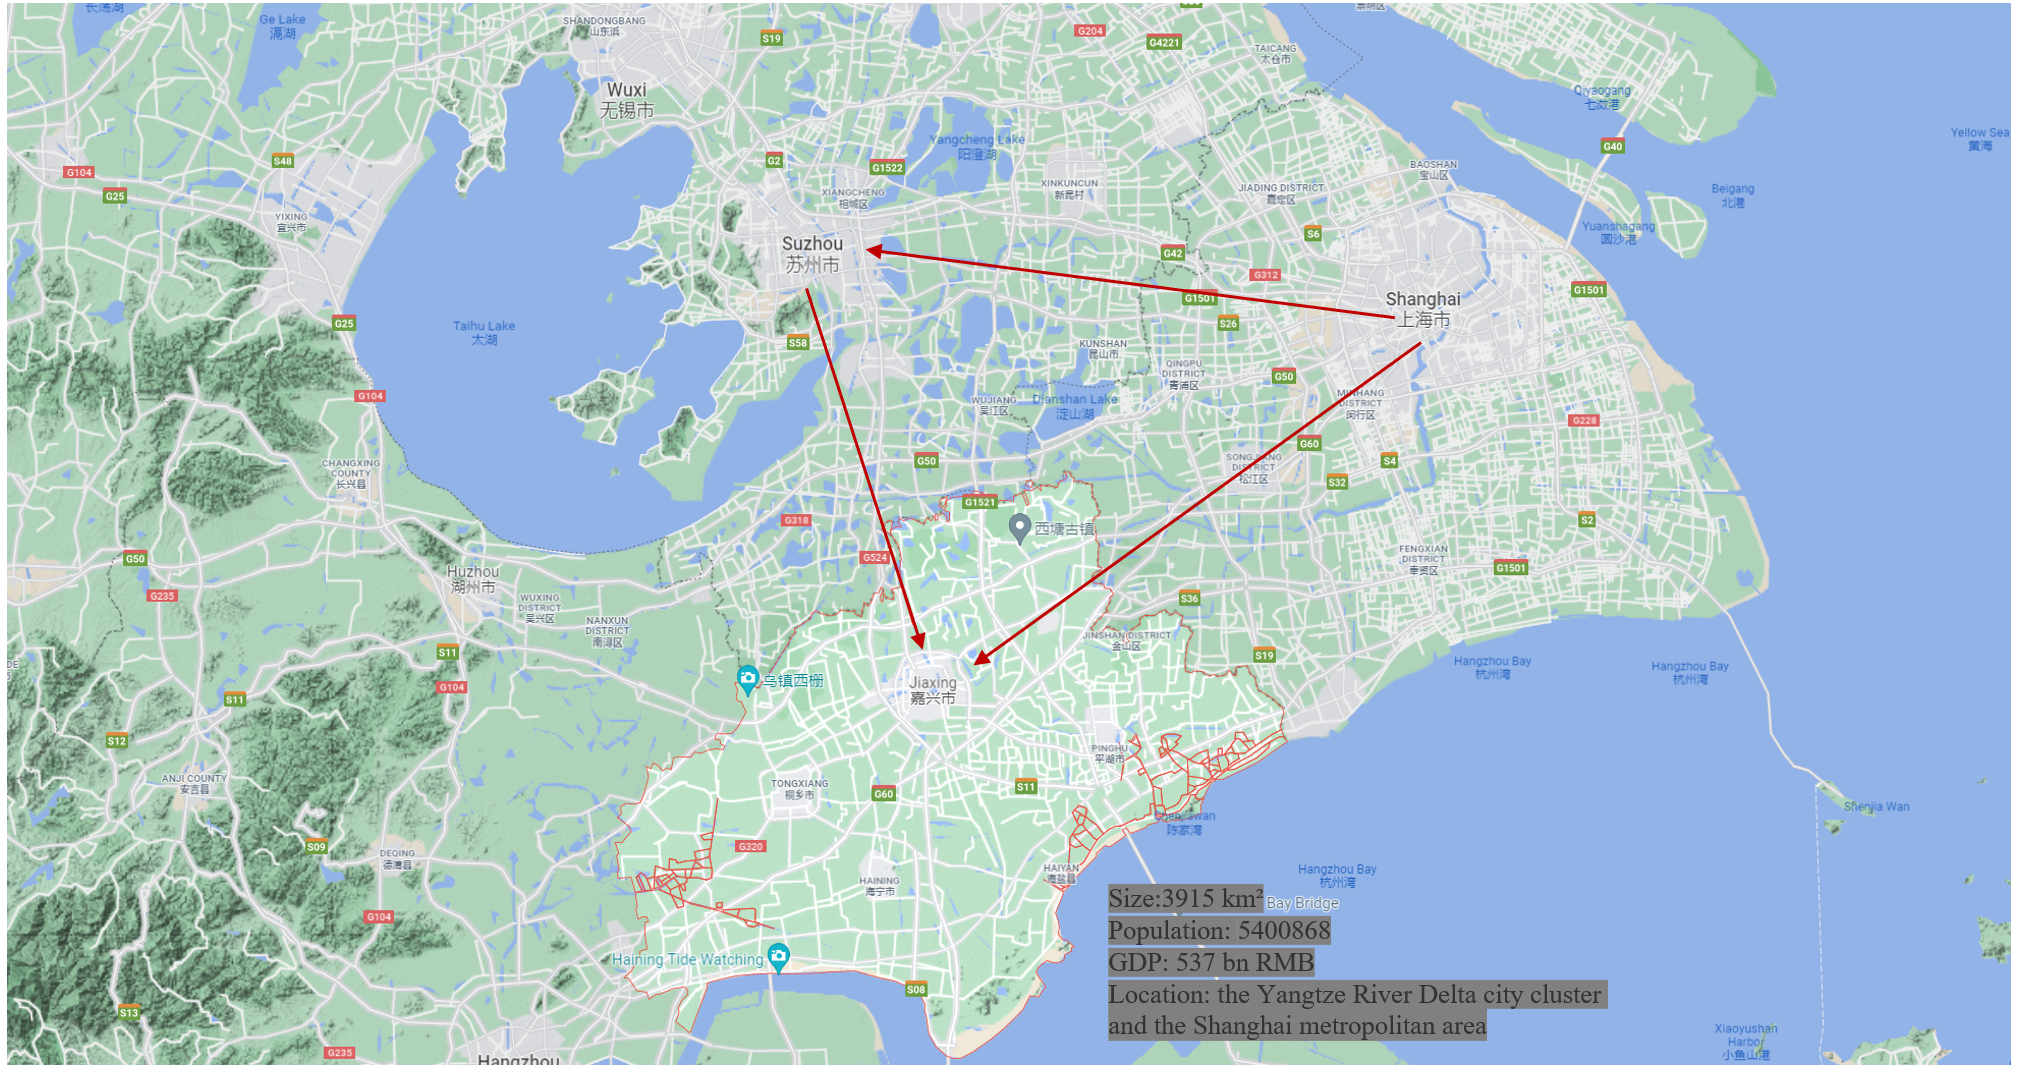
\includegraphics{maps/jiaxing.png}}
figure 5 Map of Jiaxing city in China

\hypertarget{data-collection-and-preprocess}{%
\subsection{Data collection and
preprocess}\label{data-collection-and-preprocess}}

For this research, social media data (Weibo posts) was collected from
Sina Weibo, which is one of the most used online social platform in
China. The collected Weibo posts are restricted with the tag ``Jiaxing''
in 2018, which limited the posts related to the case city. The untreated
data included a large amount of advertisements, which have been removed
by identifying certain keywords such as ``advertisement'', ``cost
performance'', etc. The urban amenity data is collected from Gaode Map
as spatial points of interest (POI). The regulatory detailed planning
(RDP) documents from 2017-2020 issued by the local government in Jiaxing
are collected from the local government office (figure 6).

\href{https://WTHSYZW.github.io/Thesis_2022/maps/RDP.png}{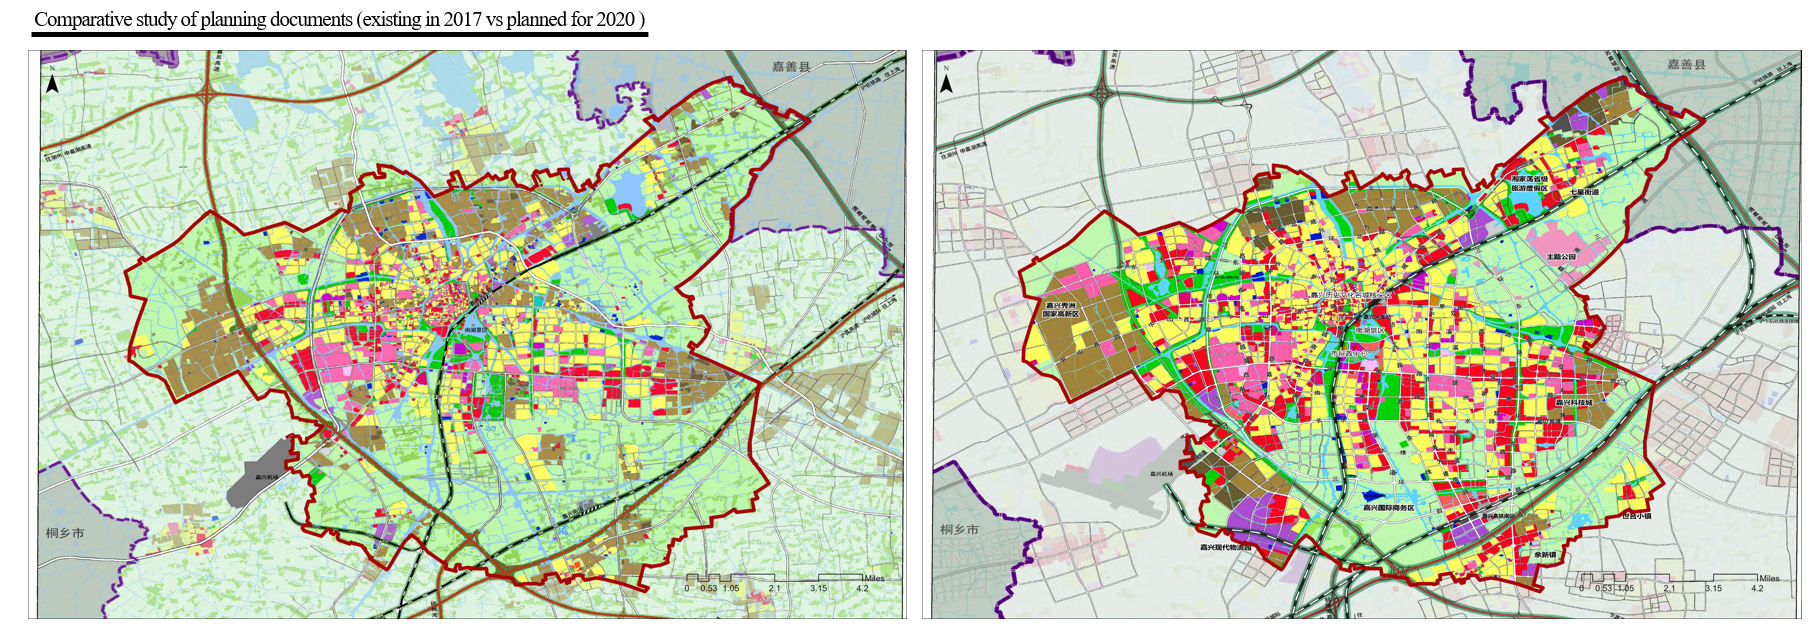
\includegraphics{maps/RDP.png}}
figure 6 RDPs of Jiaxing city in China

\hypertarget{sentiment-analysis-of-social-media-post}{%
\subsection{Sentiment analysis of social media
post}\label{sentiment-analysis-of-social-media-post}}

To study individual sentiment and its response to different built
environments, this research collects social media posts in 2018 as a
primary resource via the API of Sina Weibo. Individual emotional
preference (positive probability of individual post ) would be defined
as individual real-time feeling toward the built environment. The Baidu
AI platform has allowed researchers to analyze public sentiment via its
well-developed emotion dictionaries and its trained machine learning
model for decades in the Chinese context. Thus, the sentiment analysis
of individual posts will be conducted by accessing a machine learning
model from the Baidu AI platform. The return value of individual post
contains three parts: sentiment category, positive probability and
negative probability. In this research, the positive probability is used
to represent the probability of individual satisfaction to be positive.
The sentiment results of weibo posts are mapped as followed (figure 7).

\href{https://WTHSYZW.github.io/Thesis_2022/maps/sentiment.pdf}{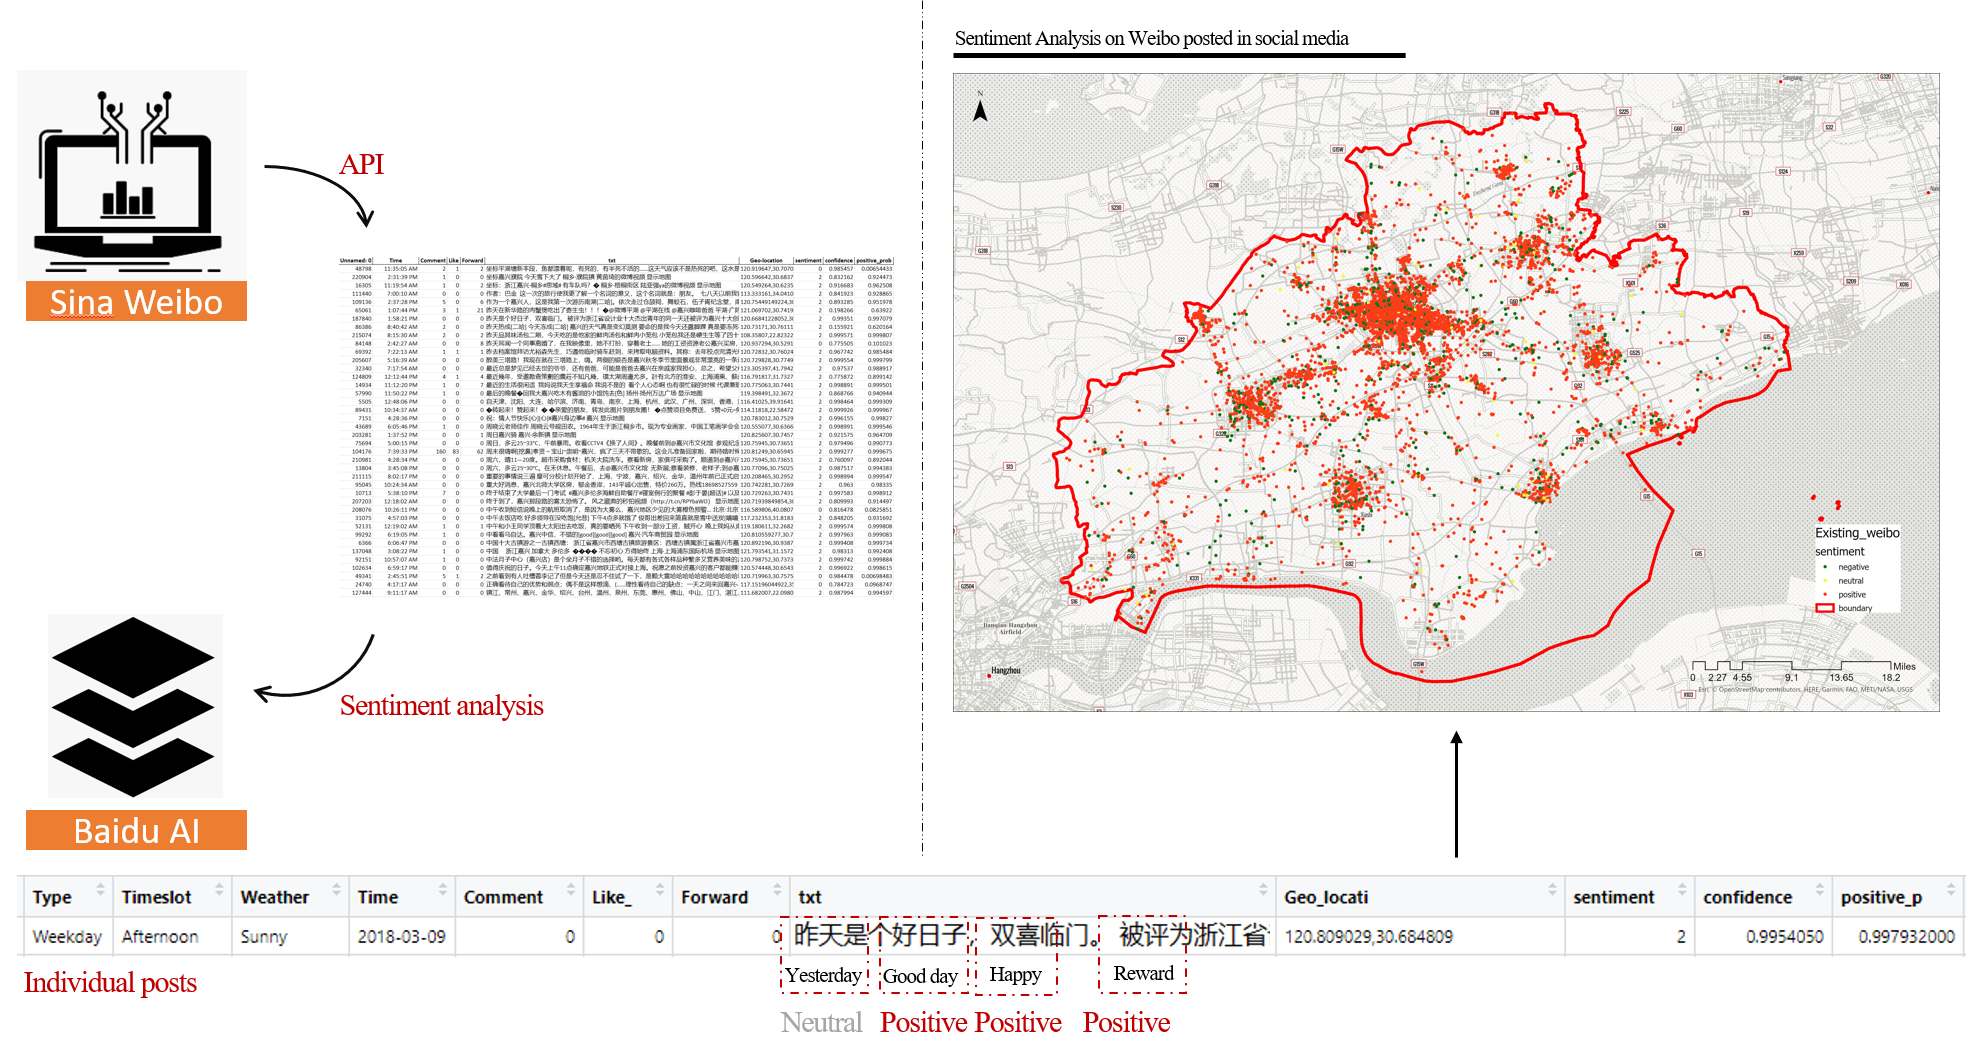
\includegraphics{maps/sentiment.png}}
figure 7 The sentiment analysis process and existing sentiment map of
Jiaxing city based on Weibo posts

\hypertarget{proximity-to-urban-amenities}{%
\subsection{Proximity to urban
amenities}\label{proximity-to-urban-amenities}}

In this research, proximity is defined by the accessibility of urban
activities and amenities by walking and by characteristics of pedestrian
networks. The amenities dataset is collected as points of interests
(POI) from Gaode Map in China, which is one of the most widely used
digital navigation systems in China (figure 8). The urban networks are
extracted from the Open Street Map (OSM). Proximity will be calculated
by the R5 package embedded in the R studio. One example of proximity to
restaurant is shown as followed (figure 9).

\href{https://WTHSYZW.github.io/Thesis_2022/maps/POI.jpg}{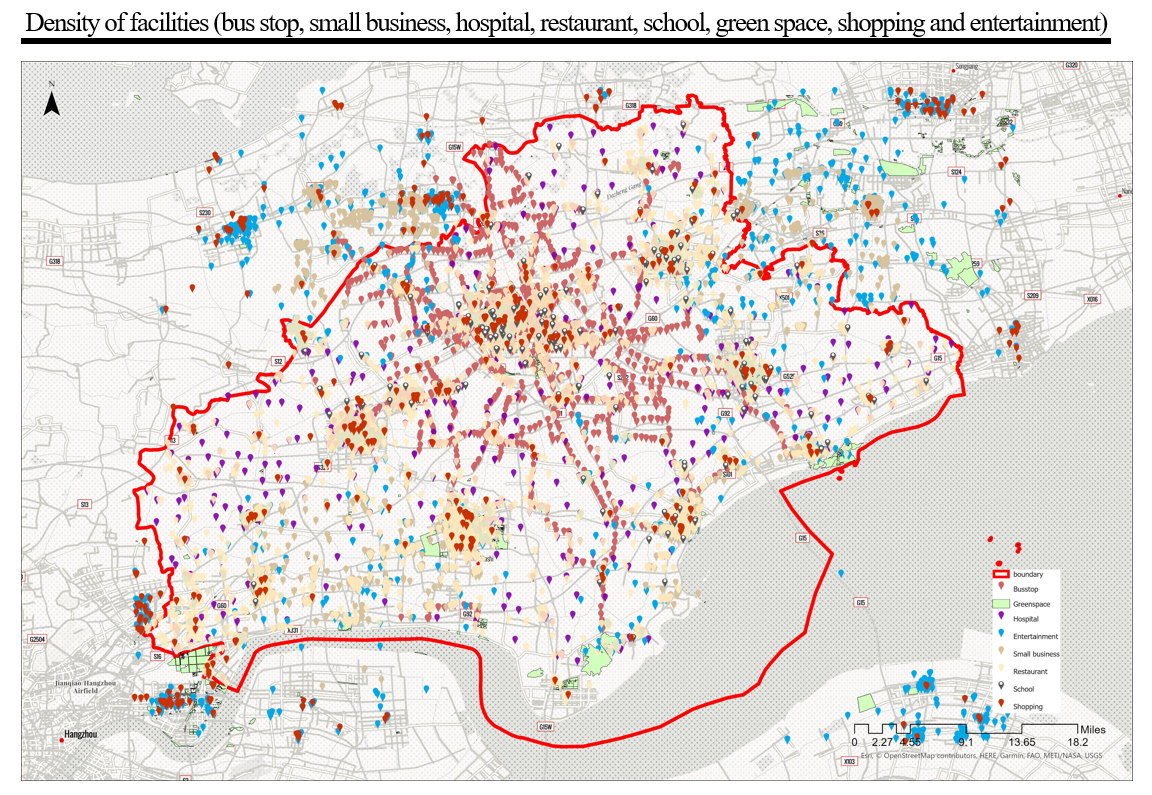
\includegraphics{maps/POI.png}}
figure 8 Density of urban amenities in Jiaxing

\href{https://WTHSYZW.github.io/Thesis_2022/maps/proximity.png}{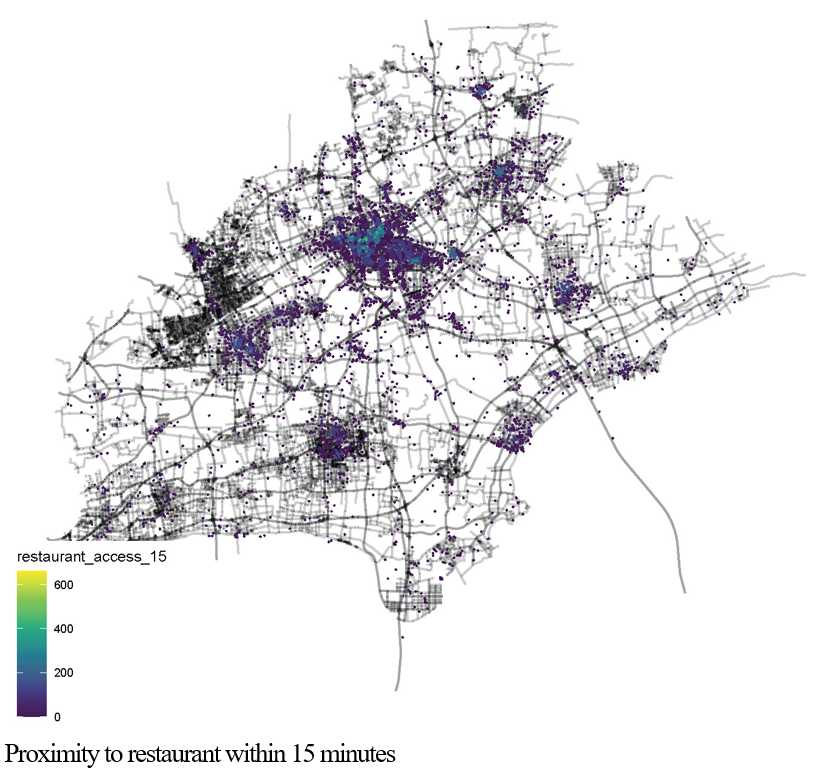
\includegraphics{maps/proximity.png}}
figure 9 Proximity to restaurant within 15 minute walking distance

\hypertarget{results}{%
\section{Results}\label{results}}

\hypertarget{correlation-between-urban-satisfaction-and-the-built-environment}{%
\subsection{Correlation between urban satisfaction and the built
environment}\label{correlation-between-urban-satisfaction-and-the-built-environment}}

To understand how the urban environment would affect individual
satisfaction from social media, a series of regression models between
sentiment results and the proximity to urban amenities were conducted.To
further improve the interpretation of regression model, the regression
analysis between sentiment result and the different proximity based on
various walking distance were applied. In addition, adding the time,
weather and workday variables helps improve the model and further
understand which variable might affect individual sentiment other than
the built environment (figure 10).

\href{https://WTHSYZW.github.io/Thesis_2022/maps/models.png}{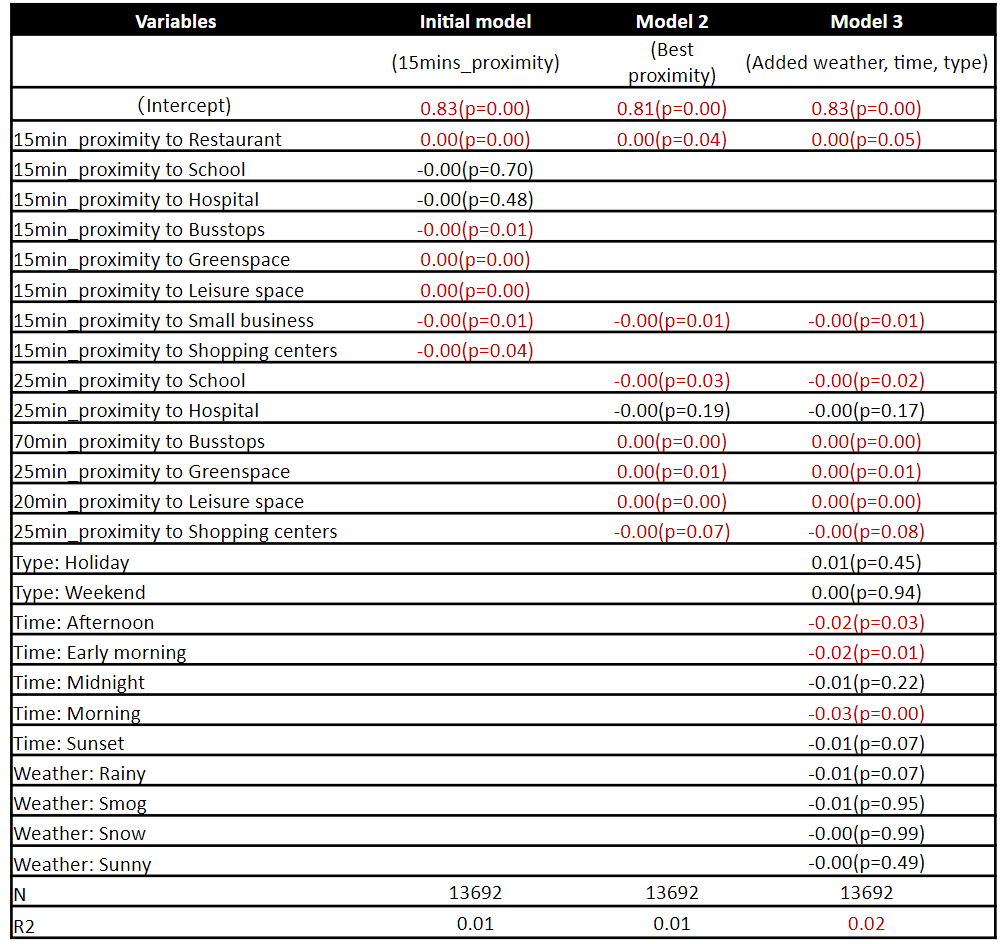
\includegraphics{maps/models.png}}
figure 10 Regression models results

\hypertarget{regression-analysis-on-the-relationship-between-individual-satisfaction-and-the-proximity-to-urban-amenities}{%
\subsection{Regression analysis on the relationship between individual
satisfaction and the proximity to urban
amenities}\label{regression-analysis-on-the-relationship-between-individual-satisfaction-and-the-proximity-to-urban-amenities}}

The regression model shows that proximity to restaurant, busstop, green
space, leisure space are positively related to individual satisfaction
on Weibo post; while the proximity to school, shopping centers and small
business are negatively related to individual satisfaction In addition,
adding the time, weather and workday variables, I found that the Time of
the weibo post in the early morning, morning and afternoon is negatively
related to individual satisfaction, while weather and workday variables
are not related to individual satisfaction (figure 11).

\href{https://WTHSYZW.github.io/Thesis_2022/maps/regression1.png}{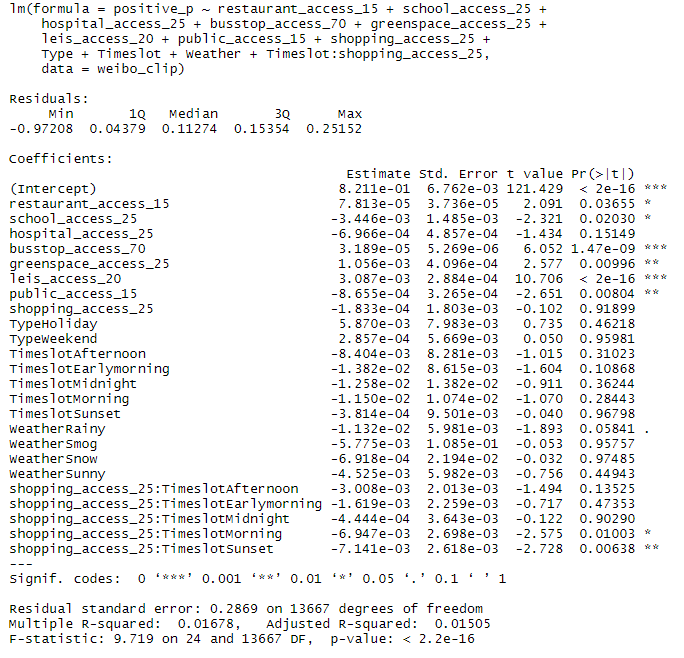
\includegraphics{maps/regression1.png}}\\
figure 11 Detailed result of regression model3

The threshold tests indicate the best fits of walking distance to
different amenities for the regression models: the proximity to
restaurant within 15 mins, the proximity to school within 25 mins, the
proximity to green space within 25 mins, the proximity to hospital
within 25 mins, the proximity to bus stops within 70 mins, the proximity
to leisure space within 20 mins, the proximity to small business within
15 mins, the proximity to shopping center within 25 mins (figure 12).

we can explore individual satisfaction and the distribution of urban
amenities in the interactive map, the darker circle represents more
positive individual satisfaction is (figure 13). The colorful dots
represent the locations of urban amenities.

\href{https://WTHSYZW.github.io/Thesis_2022/maps/bestfit.png}{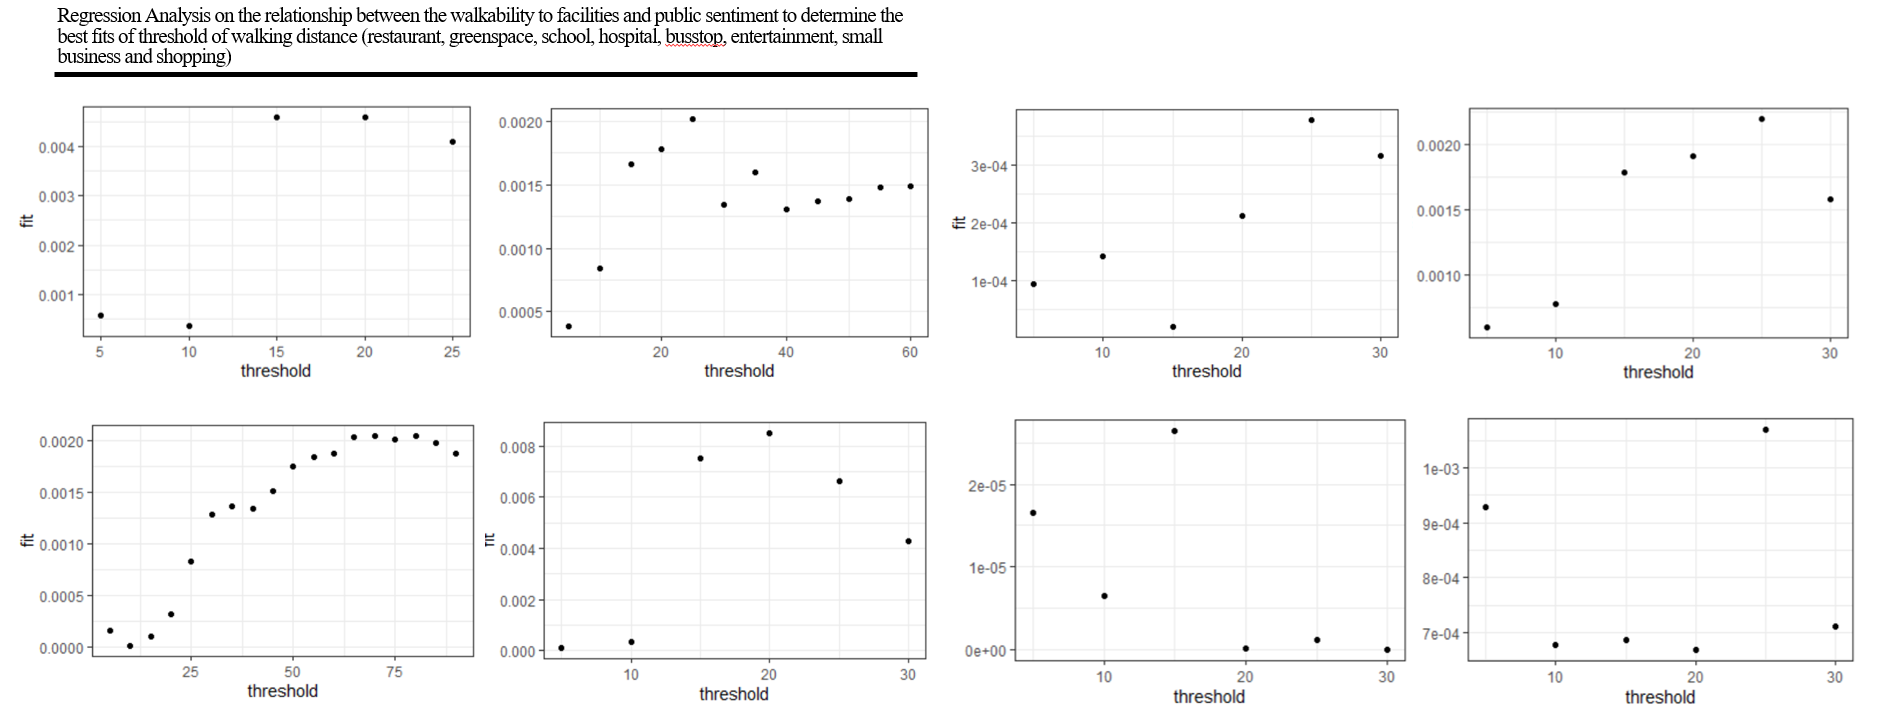
\includegraphics{maps/bestfit.png}}
figure 12 Threshold tests for the best fits of proximity to urban
amenities
\href{https://WTHSYZW.github.io/Thesis_2022/jx_ex.html}{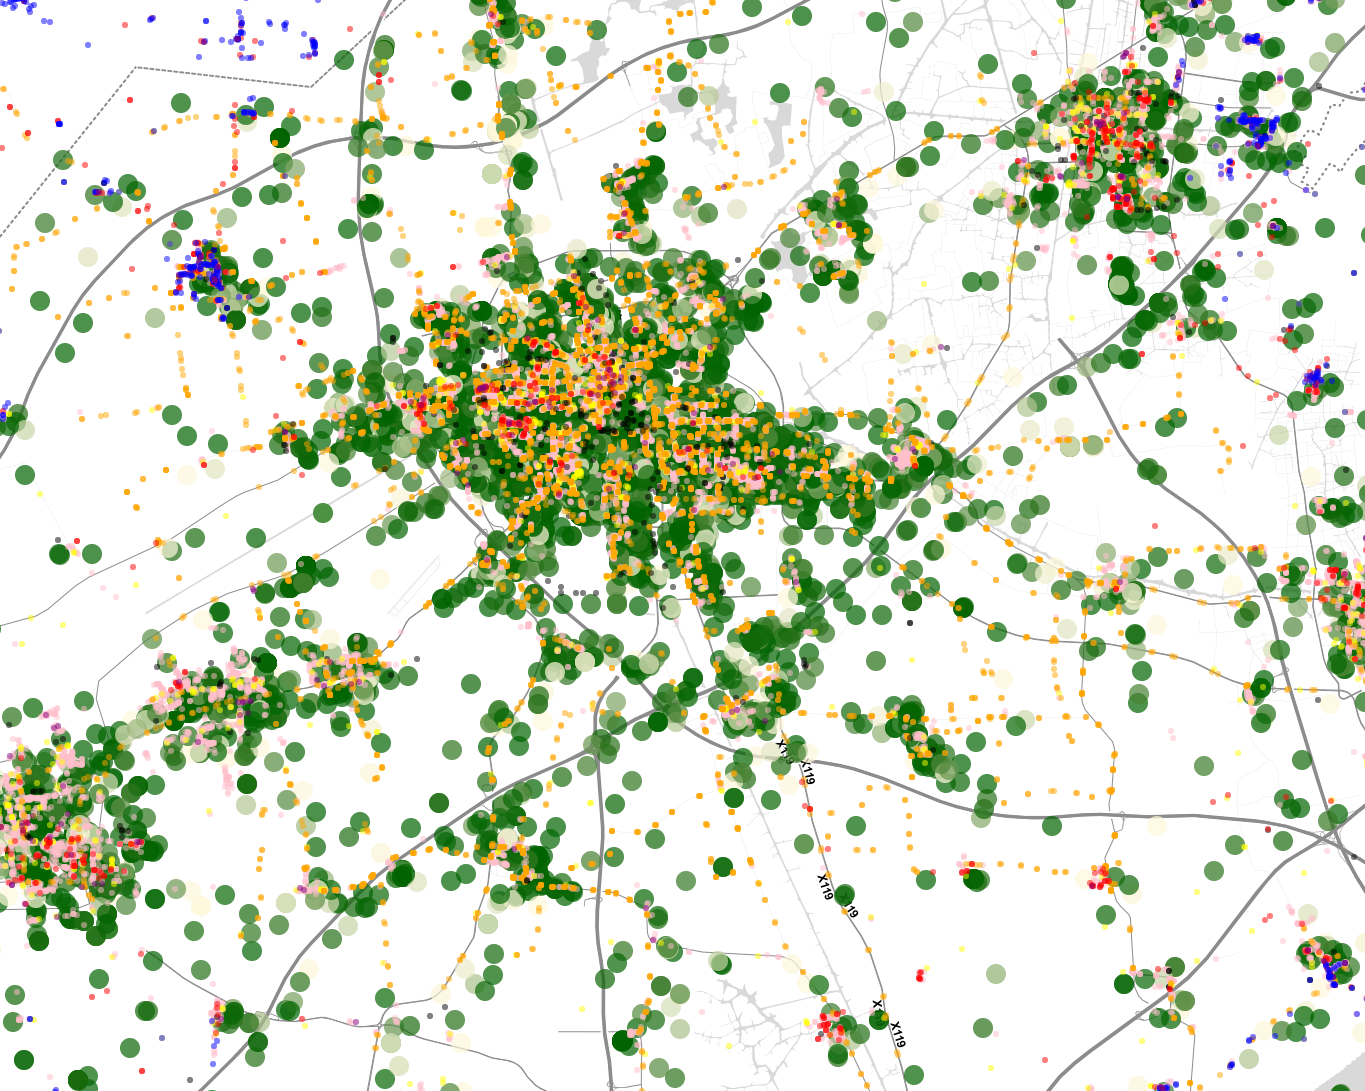
\includegraphics{maps/jx_ex.png}}
figure 13 Interactive map of existing Jiaxing

\hypertarget{prediction-of-satisfaction-changes-based-on-the-regression-model}{%
\subsection{Prediction of satisfaction changes based on the regression
model}\label{prediction-of-satisfaction-changes-based-on-the-regression-model}}

By applying the established regression model, the positive probability
of individual post can be simulated by providing a set of proximity to
urban amenities which can be calculated by the geo-locations of them.
However, what if we blindly accept this prediction model and optimize
planning decision based on the existing Weibo data?

To examine the potential and shortcomings of the simulation model, this
research provides three different planning scenarios: the official
planning documents, educational city (double the number of school) and
tourism city (replace the school with greenspace). Each scenario
associates with individual set of urban amenities, simulating different
individual sentiment map of Jiaxing. By comparing the scenarios and the
exiting condition, we could interpret how the built environment may
affect individual satisfaction in social media. More importantly, the
result demonstrates how a bad planning will be made if we optimize
public satisfaction blindly based on the existing Weibo data.

\hypertarget{scenario1}{%
\subsection{Scenario1}\label{scenario1}}

The planning scenario 1 of Jiaxing is based on the offical planning
document issued by local government (figure 14). Base on the changes of
residential and business zoning in Jiaxing, the simulation of new
restaurant locations are generated by assuming the same density of
restaurant in these zoning. After comparing of the averages of public
sentiment between the planned condition and existing condition, it was
surprising to find that the simulated future sentiment was less than the
existing sentiment result at -0.05382951. It suggests that the future
Jiaxing might not improve residents' happiness in social media.

\href{https://WTHSYZW.github.io/Thesis_2022/jx_map_scenario1.html}{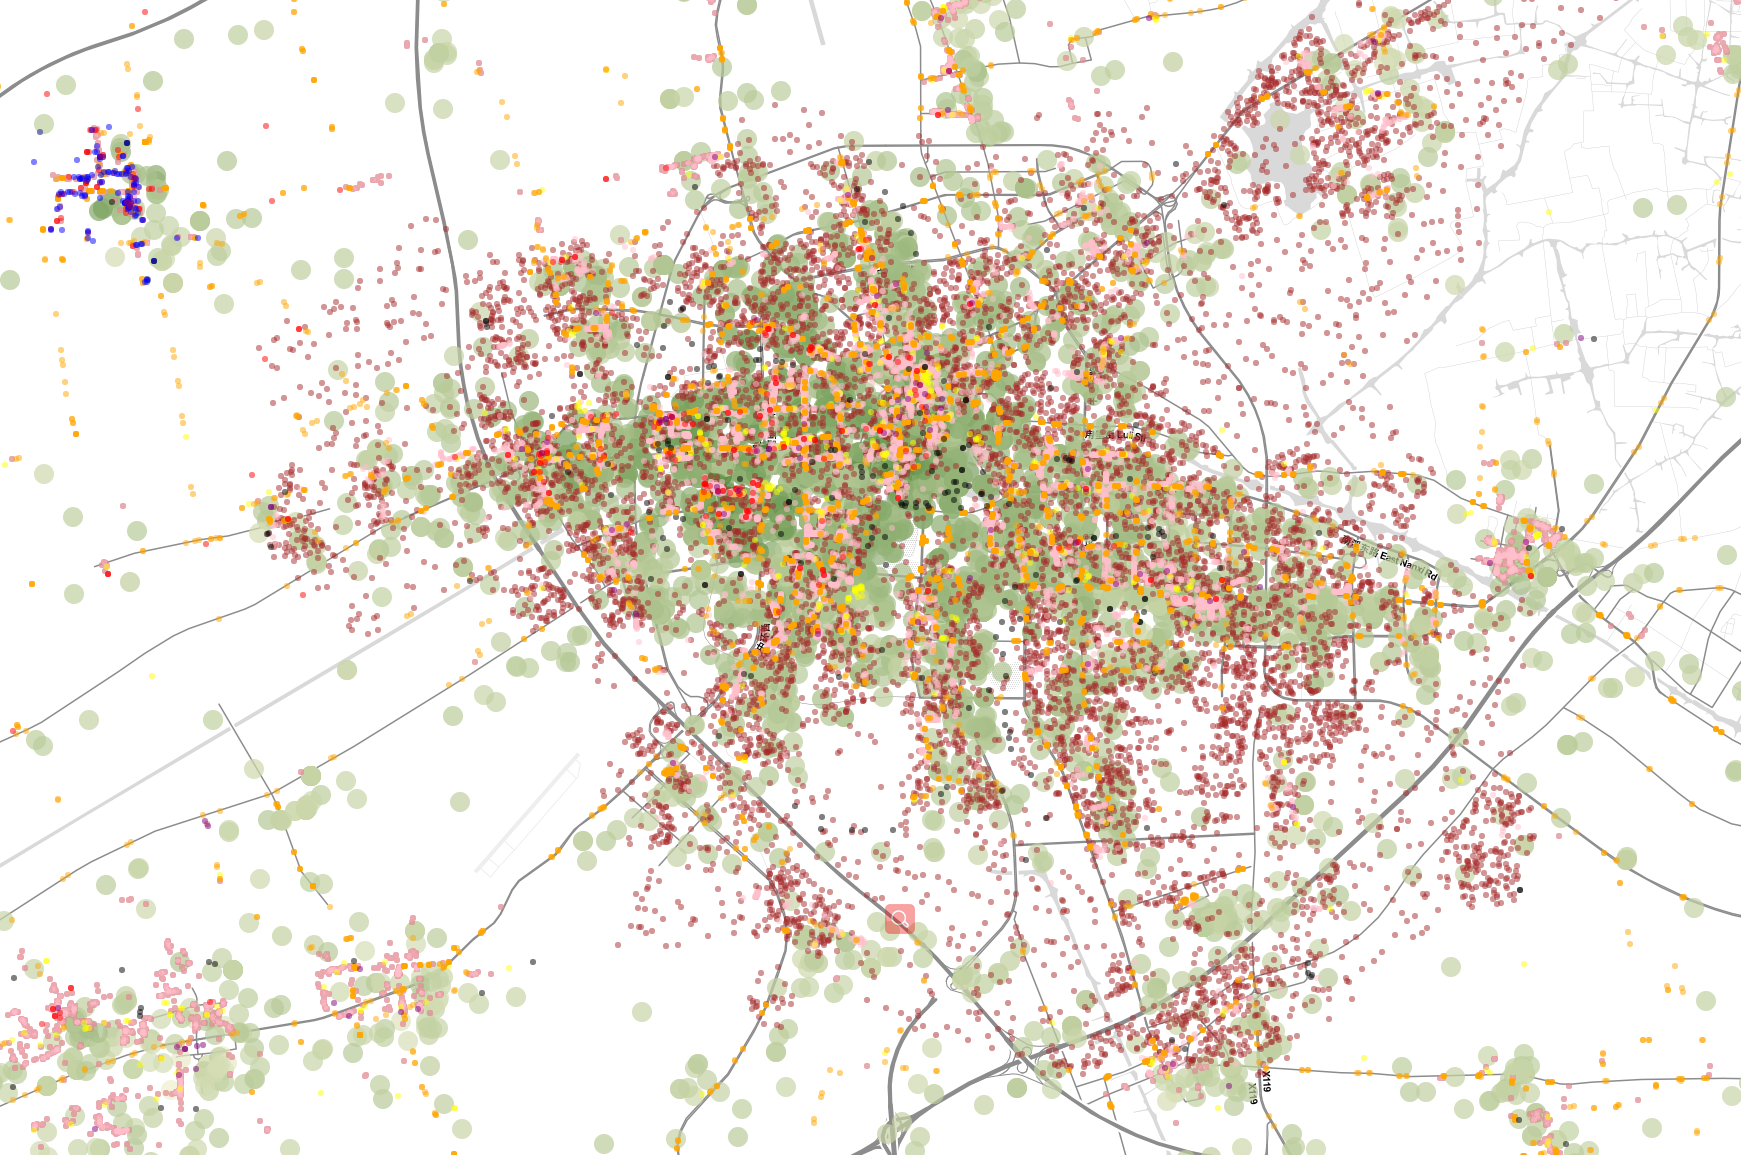
\includegraphics{maps/jx_map_scenario1.png}}
figure 14 Interactive Map of Jiaxing in Scenario 1

\hypertarget{scenario2}{%
\subsection{Scenario2}\label{scenario2}}

Scenario 2 intends to simulate an educational Jiaxing city by doubling
the number of school spreading out the city (figure 15). The original
schools remind the same locations, while randomly generating same amount
of schools spreading out the city. After comparing of the averages of
public sentiment between the scenario 2 and existing condition, the
simulated sentiment was less than the existing sentiment result at
-0.0002921917 due to the negative relationship between school and public
sentiment. This finding remains questionable; it is understandable that
people might not be happly to stay at school, however, it should play an
important role in long-term wellbeing.

\href{https://WTHSYZW.github.io/Thesis_2022/jx_map_scenario2.html}{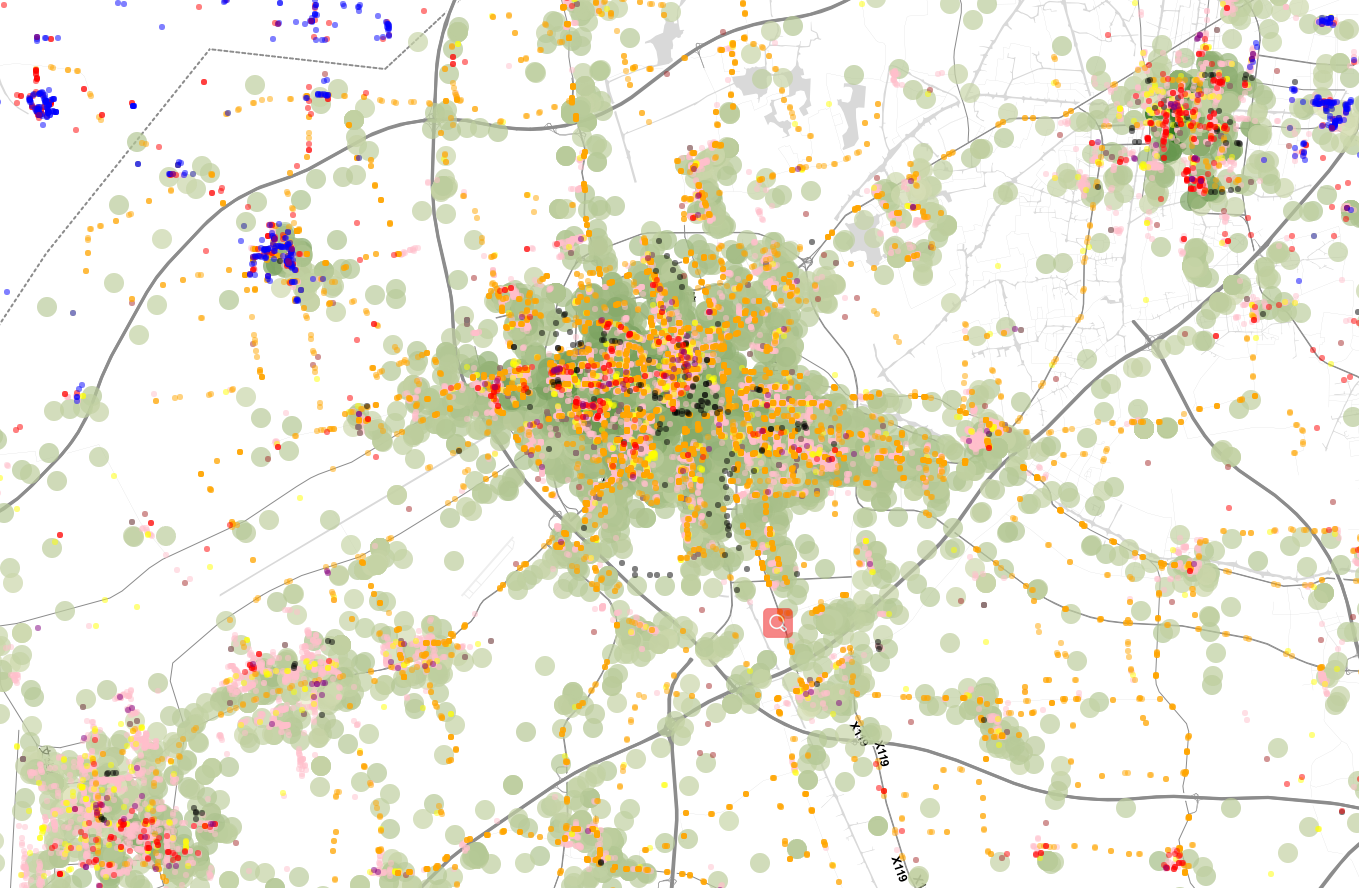
\includegraphics{maps/jx_map_scenario2.png}}
figure 15 Interactive Map of Jiaxing in Scenario 2

\hypertarget{scenario3}{%
\subsection{Scenario3}\label{scenario3}}

Scenario 3 intends to simulate an green Jiaxing city by turning school
into green space to optimize individual sentiment from social media
(figure 16). (replacing the negative places with positive places) The
planning strategy based on the negative correlation between school and
public sentiment, while a positive correlation between green space and
public sentiment, assuming a happier Jiaxing eliminating all the
school.The result shows that the simulated average sentiment was more
than the existing sentiment result at 0.005517993, which means it
``improves'' happiness by 1 percent even it does not make sense as an
urban planning strategy.

\href{https://WTHSYZW.github.io/Thesis_2022/jx_map_scenario3.html}{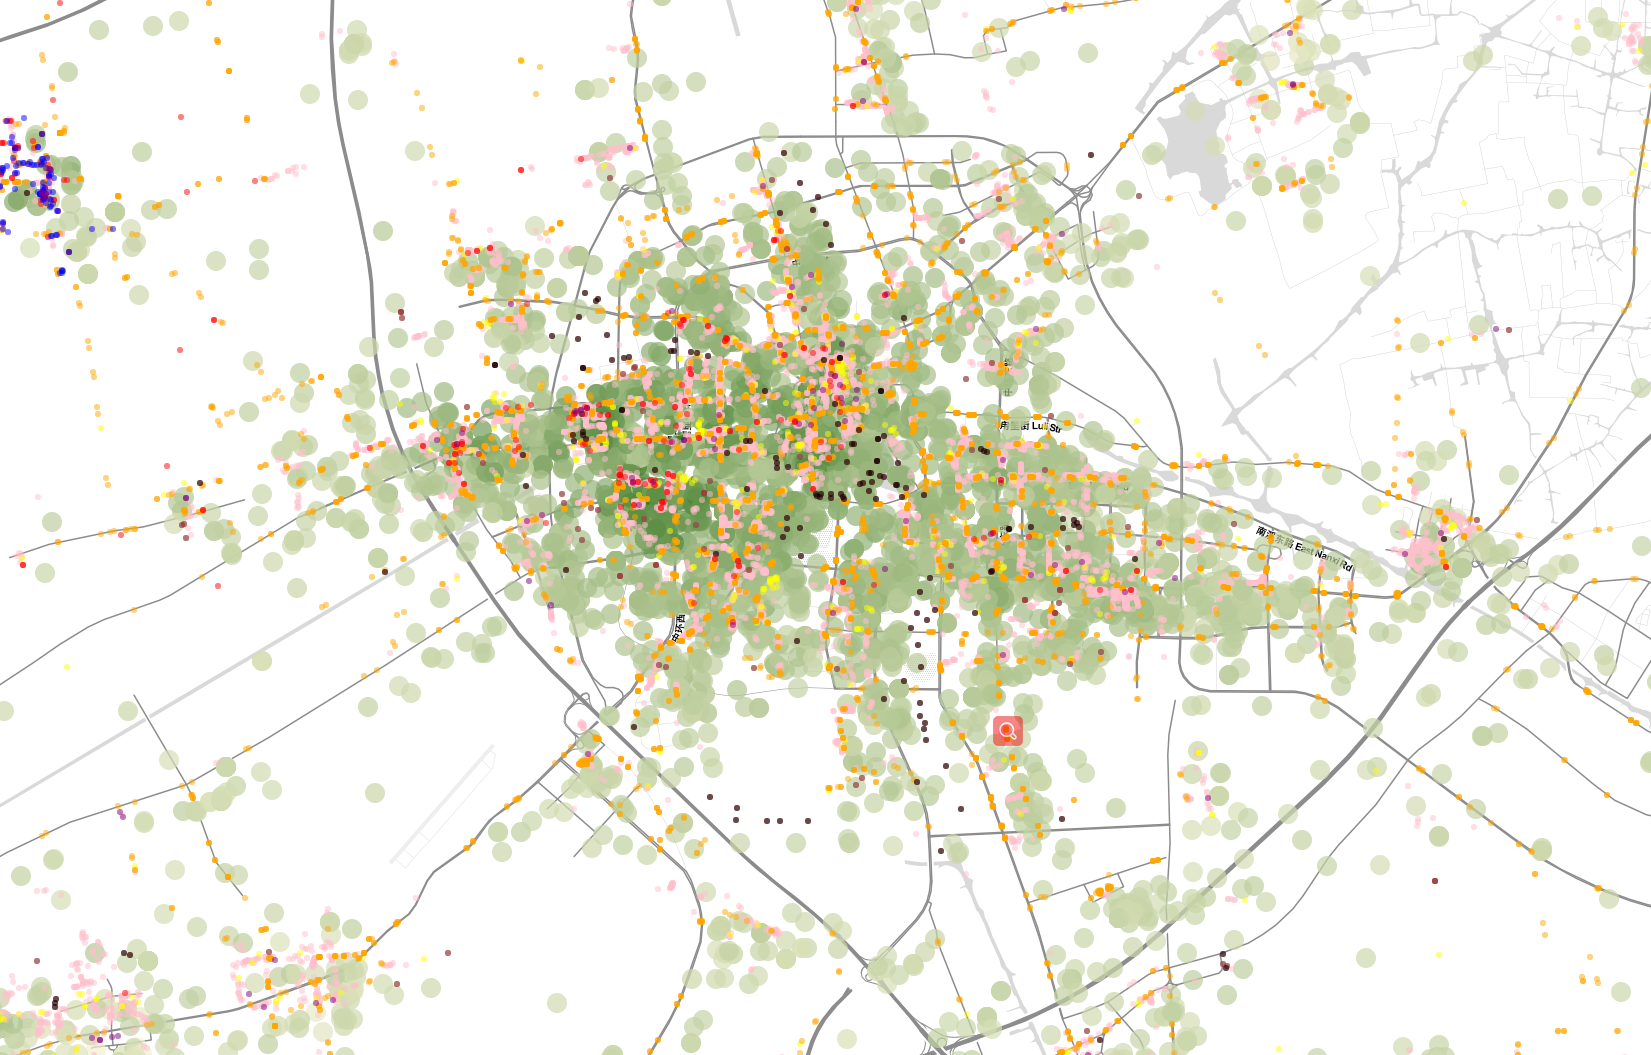
\includegraphics{maps/jx_map_scenario3.png}}
figure 16 Interactive Map of Jiaxing in Scenario 3

\hypertarget{discussion}{%
\section{Discussion}\label{discussion}}

\hypertarget{strengths-and-weaknesses-of-existing-social-media-data}{%
\subsection{Strengths and weaknesses of existing social media
data}\label{strengths-and-weaknesses-of-existing-social-media-data}}

One of the strengths of social media data is its large coverage of
population in China (figure 17). It demonstrates a prospective method
for widespread public participation that is distinct from other
traditional methods that are time-consuming and involve a small number
of representatives. The usage of social media platforms is already
embedded in people's daily lives, which facilitates public
participation, particularly for those in China who merely contributed to
urban planning process before.

\href{https://www.statista.com/statistics/277586/number-of-social-network-users-in-china/\#professional}{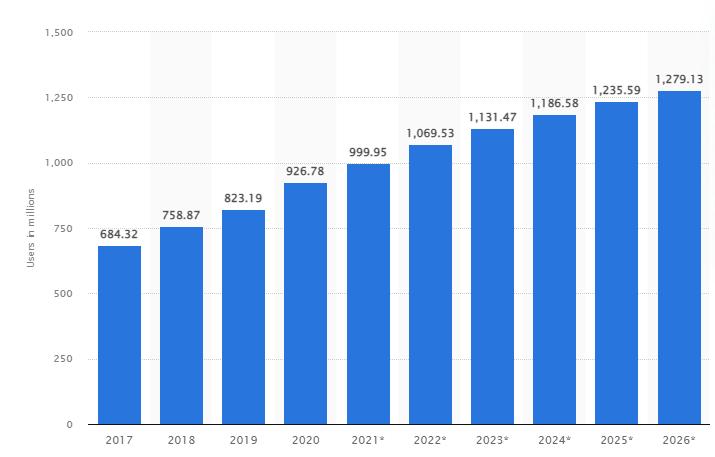
\includegraphics{maps/internet_user.png}}\\
figure 17 Number of internet population in China

However, it should be noticed that there are critical shortcomings of
the existing social media data:

\begin{itemize}
\tightlist
\item
  the existing social media data from weibo posts express short-term
  feeling rather than long-term expectation about the city;\\
\item
  the existing social media data from weibo posts are not for urban
  satisfaction in the built environment;\\
\item
  the existing social media data from weibo posts are passively engage
  in data-driven planning for urban satisfaction.
\item
  the existing social media data from weibo posts are subject to the
  relevant social platform so as to the targeted groups of people.
\end{itemize}

\hypertarget{inherent-conflict-between-short-term-feeling-and-long-term-urban-planning-process}{%
\subsection{Inherent conflict between short-term feeling and long-term
urban planning
process}\label{inherent-conflict-between-short-term-feeling-and-long-term-urban-planning-process}}

After a careful investigation of weibo posts, we can see that the texts
mainly represents individual real-time feelings, which implied shot-term
sentiments or comments last for minutes even seconds. However, urban
planning takes years and decades and has a long-term impact on people's
lives, which requires people's long-term expectation of cities they live
in. There appears to be an inherent conflict between them. The
discussion section on planning scenarios indicates clearly that
designing a city solely to promote short-term feelings will not result
in a better long-term well-being (especially if we replace all the
schools and hospitals with green spaces).

In comparison, the ideal data should be able to represent what people
want in the future, namely long-term expectations; how they feel about
the existing city, the satisfaction; and they should know and actively
participate in (figure 18).

\href{https://WTHSYZW.github.io/Thesis_2022/maps/comparison2.png}{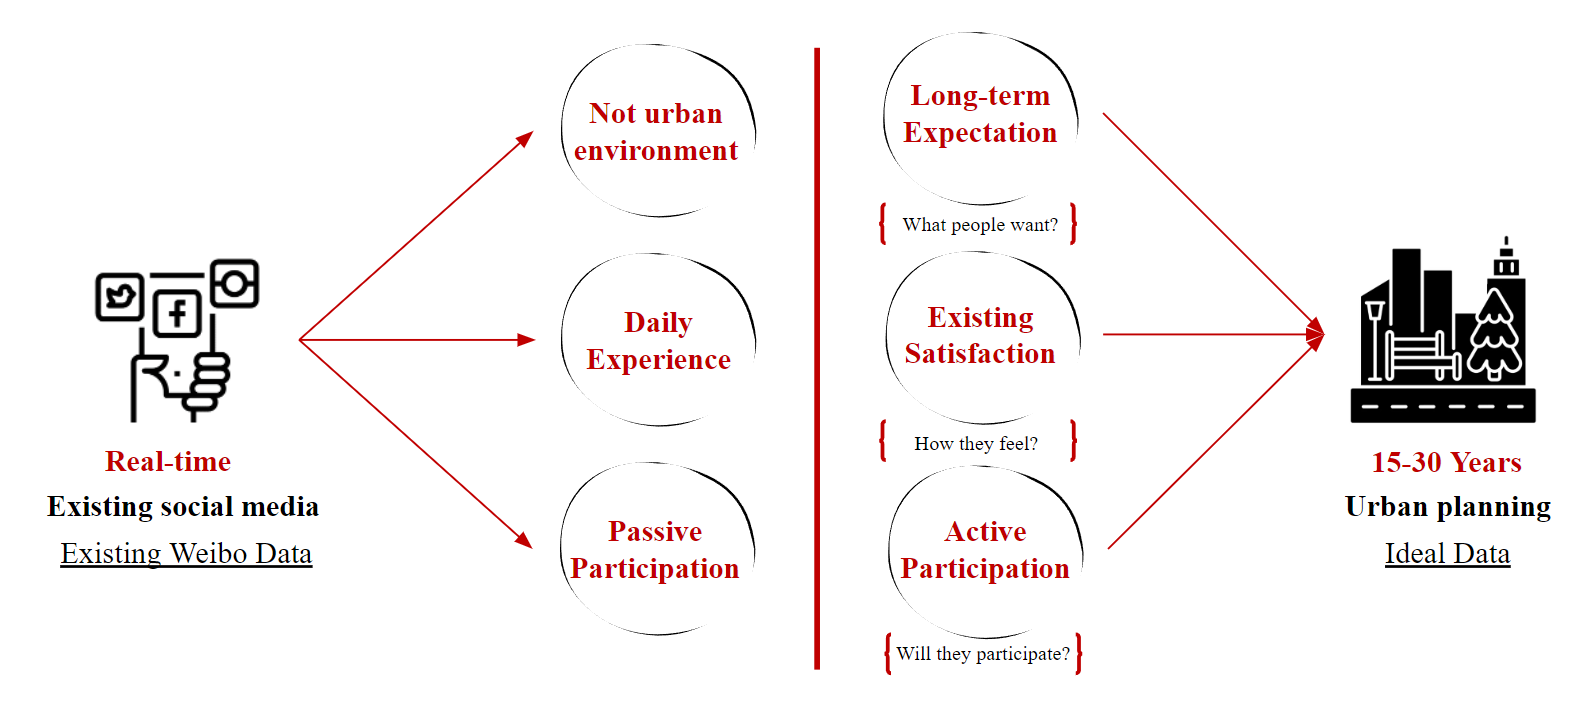
\includegraphics{maps/comparison2.png}}
figure 18 How ideal data should address the shortcomings of existing
social media data

\hypertarget{recommendation-a-proposed-social-media-platform}{%
\section{Recommendation: A proposed social media
platform}\label{recommendation-a-proposed-social-media-platform}}

How could we design A better data gathering tool?

Social media platform serves as a new form of infrastructure of urban
life, which is embedded in daily experience.The strengths of such social
media platform can provide a mass bottom-up participation that
traditional approaches can not provide. To address the shortcomings of
existing social media data, the new social media platform should be
capable of providing particular data on short-term satisfaction related
to the built environment and long-term visions of urban planning from
citizens living in that city.\\
Thus, I propose a new social media platform that can collect
geo-location, long-term expectation, daily comments and satisfaction of
the built environment of individuals, which can provide precise data for
proposed quantitative methodology (figure 19).

\href{https://WTHSYZW.github.io/Thesis_2022/maps/app2.png}{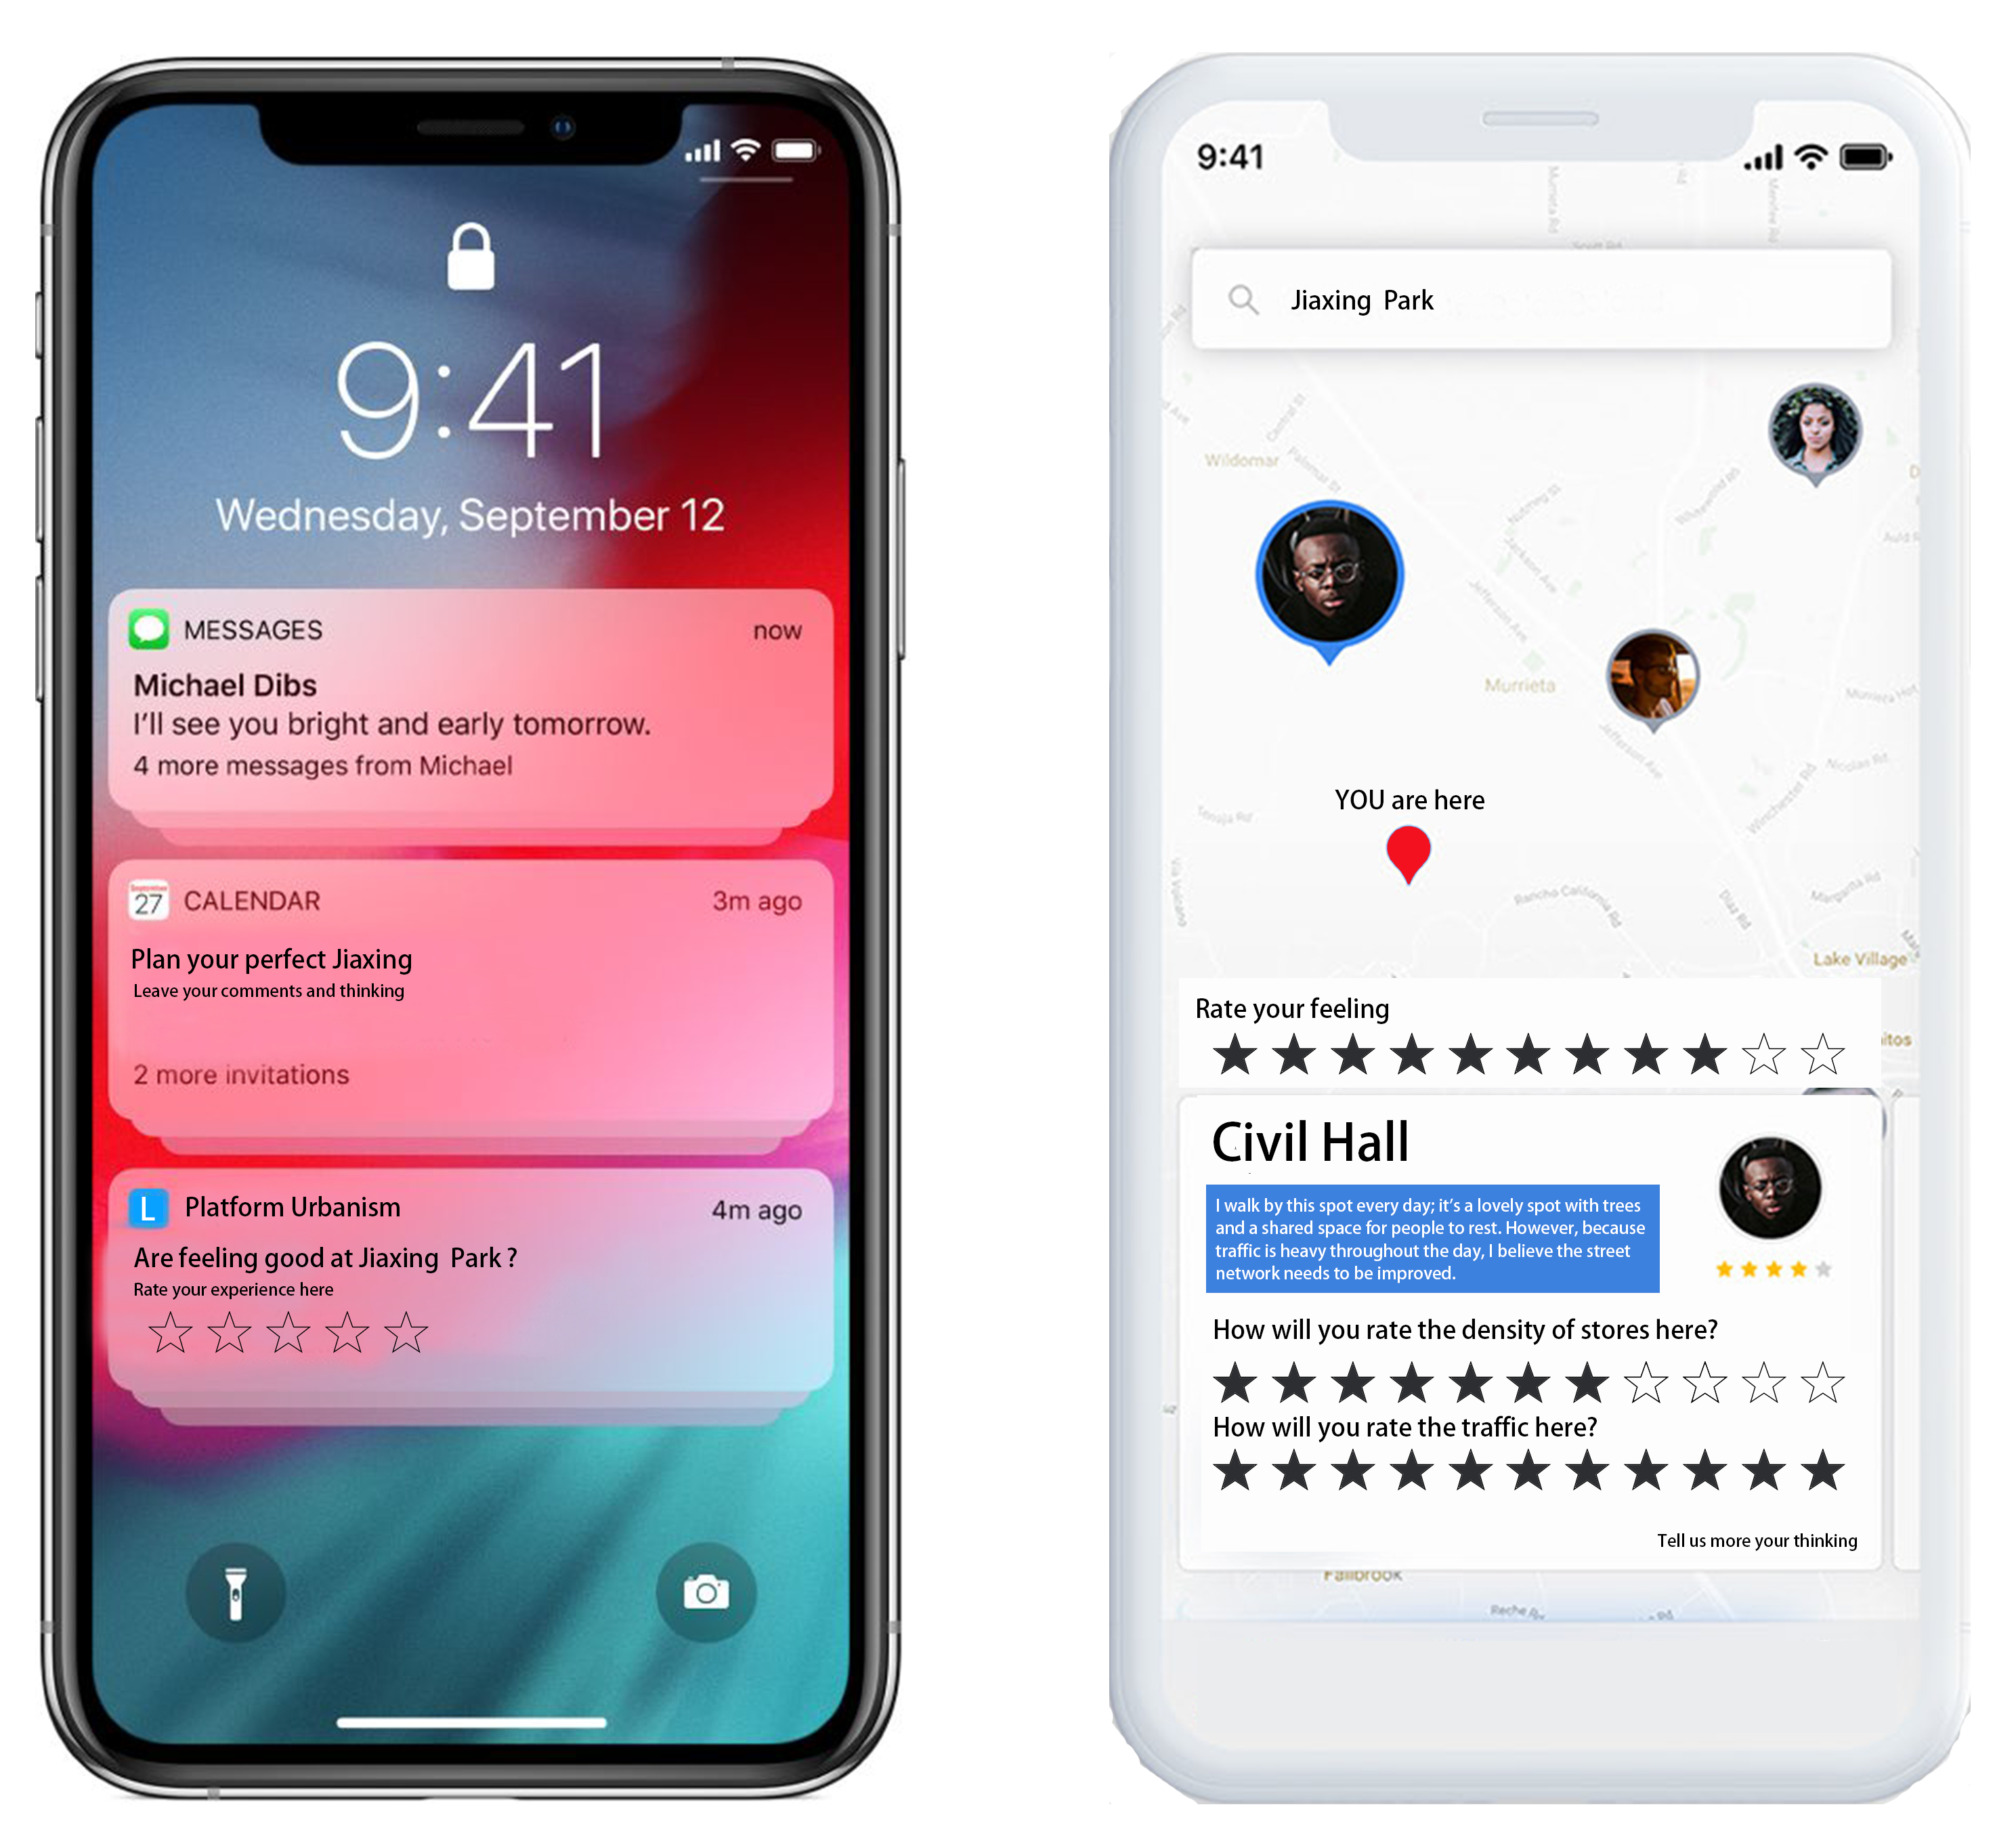
\includegraphics{maps/app2.png}}\\
figure 19 A proposed new social media platform

To collect such data, a series of quantitative questions will be asked
whenever users want to rate the characteristics of the built
environment. People can actively express their feeling and comments
about the space, and interact with others thoughts on this new social
media platform (figure 20). In addition, a notification will pop up when
people visit a urban facility such as a park, requiring a simple rating
of feeling. What is more, throughout the new urban planning process, the
government can announce a routine of public events in which it invites
public participation and citizen long-term visions for developing their
ideal city (figure 21). A social media platform is proposed as following
vision:

\href{https://WTHSYZW.github.io/Thesis_2022/maps/app3.png}{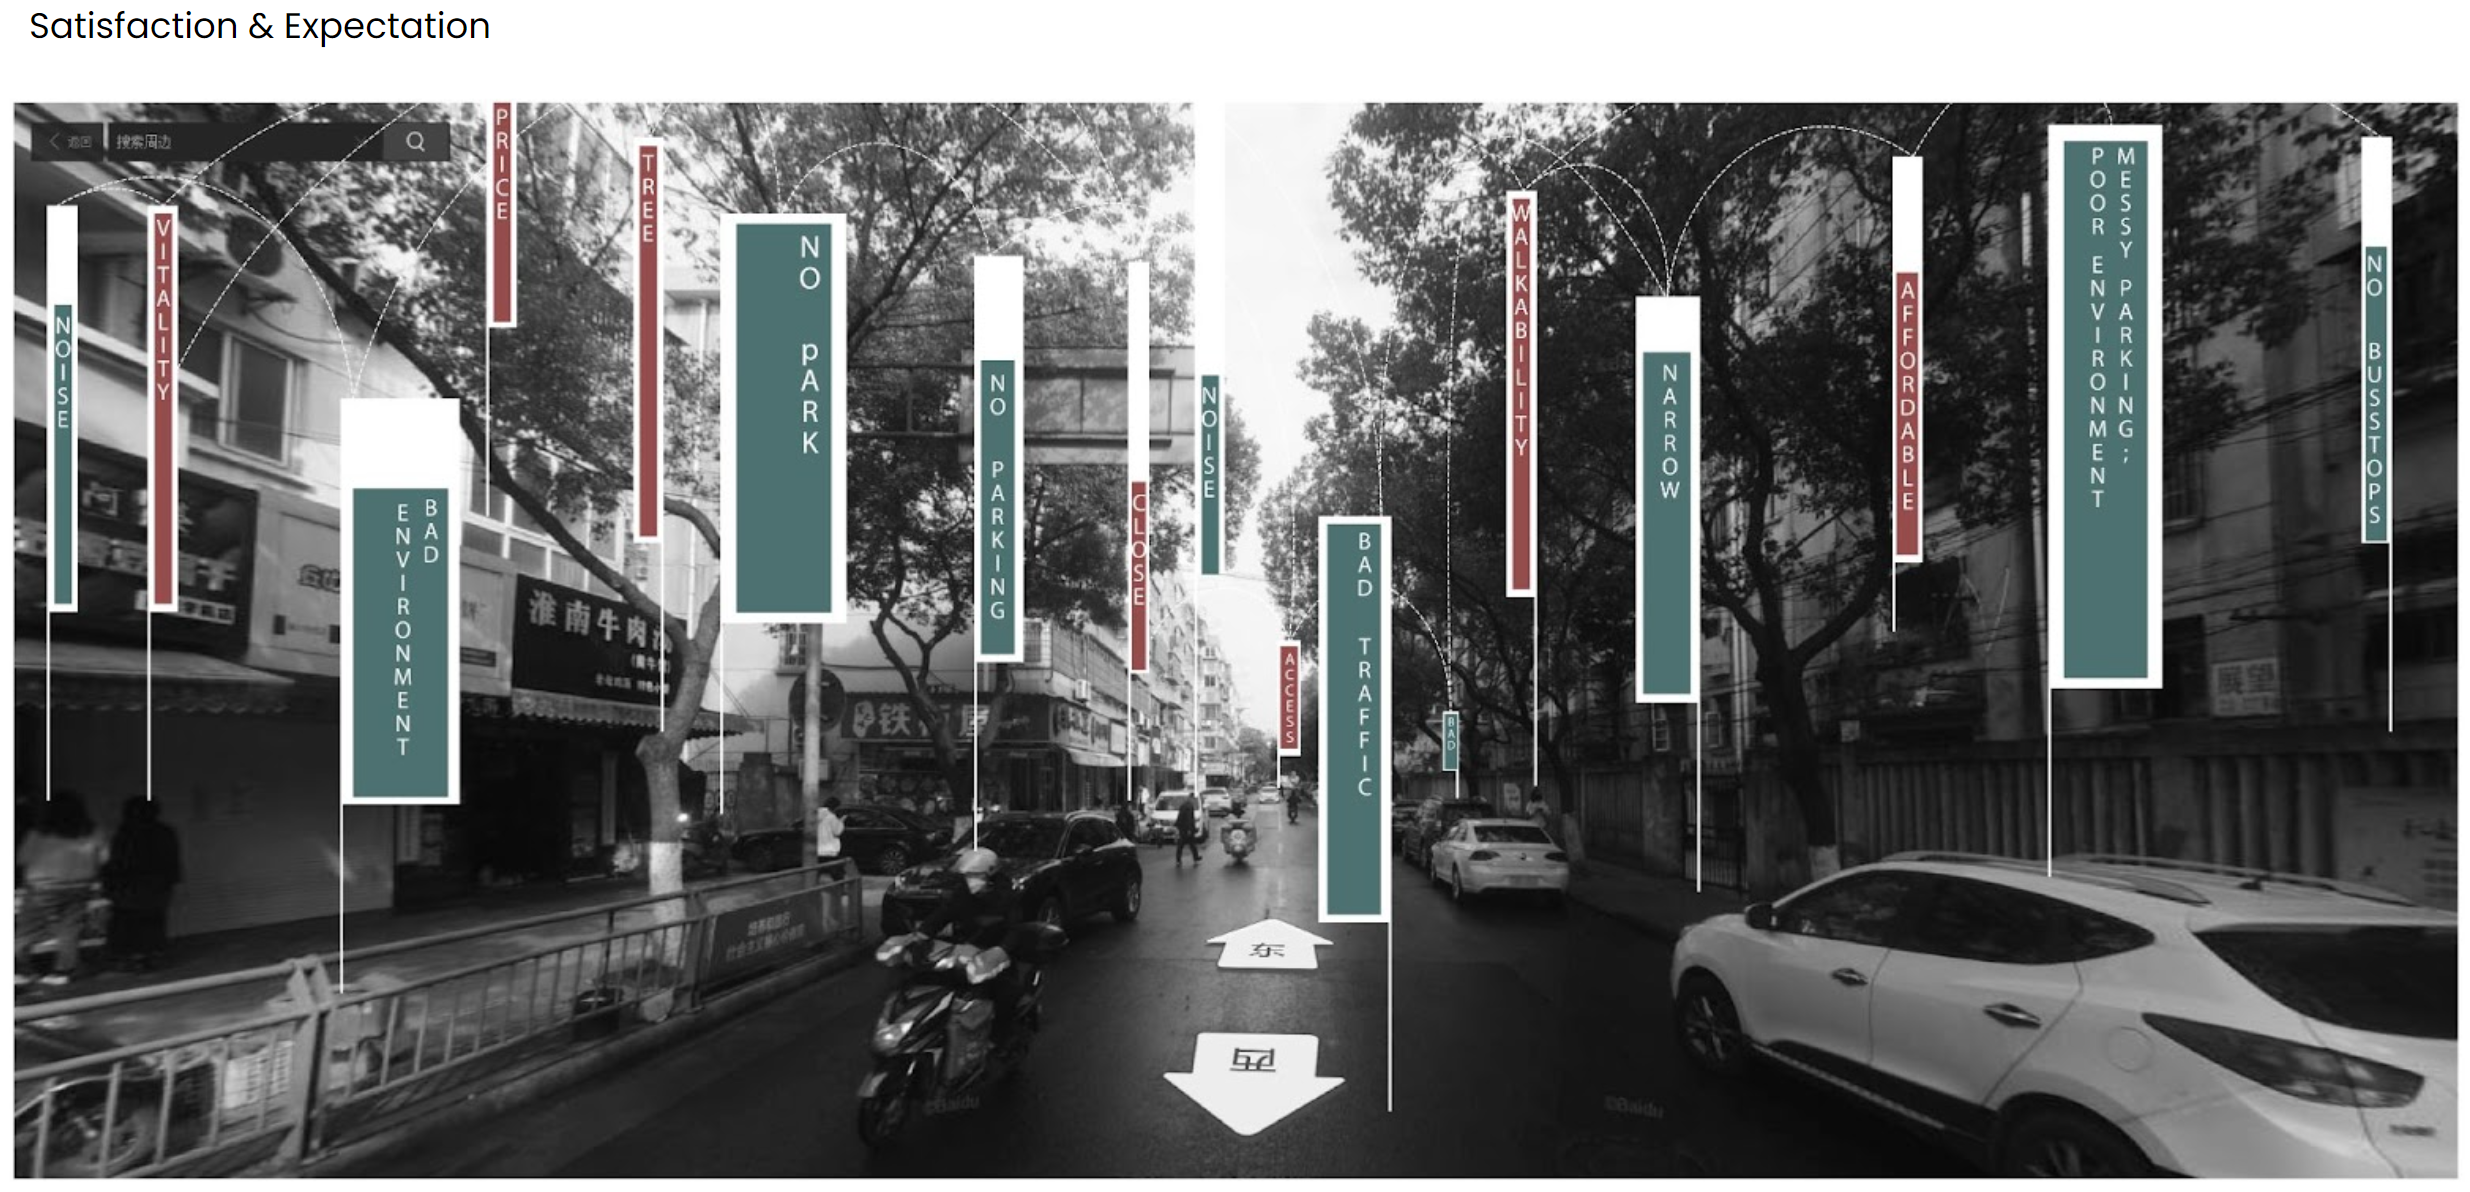
\includegraphics{maps/app3.png}}\\
figure 20 User interactions on existing urban conduction
\href{https://WTHSYZW.github.io/Thesis_2022/maps/app4.png}{\includegraphics{maps/app4.png}}\\
figure 21 User interactions on future urban conduction

\hypertarget{conclusion}{%
\section{Conclusion}\label{conclusion}}

This research shows:

\begin{itemize}
\tightlist
\item
  Serious limitations of existing social media data for data-driven
  planning.\\
\item
  Statistic significant relationships between public sentiment and the
  proximity to amenities, which proves my hypothesis that the built
  environment might affect individual sentiment;\\
\item
  A potential to help planner understand which characteristics of the
  built environment may improve residents' satisfaction;\\
\item
  A quantitative framework to quantify urban experience from text-based
  information and build a simulation model based on that;\\
\item
  New social media platform to invite mass public participation and
  data-driven urban planning;\\
\item
  New social media platform as a new form of infrastructure of urban
  life, which might bring a great potential to design a more
  people-oriented city or a new urban form.
\end{itemize}

\hypertarget{reference}{%
\section{Reference}\label{reference}}

\begin{enumerate}
\def\labelenumi{\arabic{enumi})}
\tightlist
\item
  Cervero, R., \& Kockelman, K. (1997). Travel demand and the 3Ds:
  Density, diversity, and design. Transportation research part D:
  Transport and environment, 2(3), 199-219.
\item
  Conway, J. R., Lex, A., \& Gehlenborg, N. (2017). UpSetR: an R package
  for the visualization of intersecting sets and their properties.
  Bioinformatics.
\item
  Diener, E., Suh, E. M., Lucas, R. E., \& Smith, H. L. (1999).
  Subjective well-being: Three decades of progress. Psychological
  bulletin, 125(2), 276.
\item
  DataReportal. (2022). DIGITAL 2022: CHINA.Retrieved from
  \url{https://datareportal.com/reports/digital-2022-china\#}:\textasciitilde:text=Internet\%20use\%20in\%20China\%20in\%202022\&text=China's\%20internet\%20penetration\%20rate\%20stood,percent)\%20between\%202021\%20and\%202022.
\item
  Ewing, R., \& Cervero, R. (2001). Travel and the built environment: a
  synthesis. Transportation research record, 1780(1), 87-114.
\item
  Ewing, R., \& Cervero, R. (2010). Travel and the built environment: A
  meta-analysis. Journal of the American planning association, 76(3),
  265-294.
\item
  Ewing, R., Greenwald, M. J., Zhang, M., Walters, J., Feldman, M.,
  Cervero, R., \& Thomas, J. (2009). Measuring the impact of urban form
  and transit access on mixed use site trip generation rates---Portland
  pilot study. US Environmental Protection Agency, Washington, DC.
\item
  Florida, R., Mellander, C., \& Rentfrow, P. J. (2013). The happiness
  of cities. Regional studies, 47(4), 613-627.
\item
  Guan, CH. \& Rowe, P.G. (2016). The concept of urban intensity and
  China's townization policy: Cases from Zhejiang Province. Cities. 55.
  22-41.
\item
  Gim, T. H. T. (2021). Comparing Happiness Determinants for Urban
  Residents A Partial Least Squares Regression Model. International
  Review for Spatial Planning and Sustainable Development, 9(2), 24-40.
\item
  Hogertz, C. (2010). Emotions of the urban pedestrian: sensory mapping.
  Pedestrians' quality needs, 31, 31-52.
\item
  Lawless, N. M., \& Lucas, R. E. (2011). Predictors of regional
  well-being: A county level analysis. Social Indicators Research,
  101(3), 341-357.
\item
  Leyden, K. M., Goldberg, A., \& Michelbach, P. (2011). Understanding
  the pursuit of happiness in ten major cities. Urban affairs review,
  47(6), 861-888.
\item
  Li, SJ., Ma, S., Zhang M., Long Y. (2018). Muiti-scale Evaluation of
  Urban Green Space Based on Muti-source New Data:Exploration of Main
  Cities in China. Landscape Architecture.
\item
  Ma, Y., Ling, C., \& Wu, J. (2020). Exploring the Spatial Distribution
  Characteristics of Emotions of Weibo Users in Wuhan Waterfront Based
  on Gender Differences Using Social Media Texts. ISPRS International
  Journal of Geo-Information, 9(8), 465.
\item
  Mouratidis, K. (2018). Rethinking how built environments influence
  subjective well-being: A new conceptual framework. Journal of
  Urbanism: International Research on Placemaking and Urban
  Sustainability, 11(1), 24-40.
\item
  OECD Better Life Index. How's Life? 2020 Measuring Well-Being; OECD
  Publishing: Paris, France, 202Jiang, GH., Ma, WQ., Wang, DQ., Zhou,
  DY., Zhang, RJ., \& Zhou, T. (2017). Identifying the internal
  structure evolution of urban built-up land sprawl (UBLS) from a
  composite structure perspective: A case study of the Beijing
  metropolitan area, China. Land Use Policy, 62, 258-267.
\item
  Orii, L., Alonso, L., \& Larson, K. (2020). Methodology for
  Establishing Well-Being Urban Indicators at the District Level to be
  Used on the CityScope Platform. Sustainability, 12(22), 9458.
\item
  Plunz, R. A., Zhou, Y., Vintimilla, M. I. C., Mckeown, K., Yu, T.,
  Uguccioni, L., \& Sutto, M. P. (2019). Twitter sentiment in New York
  City parks as measure of well-being. Landscape and urban planning,
  189, 235-246.
\item
  Rowe, P. G., \& Kan, H. Y. (2014). Urban Intensities: Contemporary
  Housing Types and Territories. Birkhäuser.
\item
  Rath, T., Harter, J. K., \& Harter, J. (2010). Wellbeing: The five
  essential elements. Simon and Schuster.
\item
  State Council of China. (2010). The Sixth National Census. Xinhua News
  Agency.
\item
  State Council of China. (2014). New Urbanization (citization and
  townization) Policy. Xinhua News Agency.
\item
  Song, Y., \& Gerrit-Jan, K. (2004). Measuring urban form. American
  Planning Association. Journal of the American Planning Association,
  70, 210--225.
\item
  Sun, S. (2017). On Urban Planning System in China, URP 1, 16-25.
\item
  Shen, Y., \& Karimi, K. (2016). Urban function connectivity:
  Characterisation of functional urban streets with social media
  check-in data. Cities, 55, 9-21.
\item
  Tsai, Y. (2005). Quantifying urban form: Compactness versus
  ``sprawl''. Urban Studies, 42(1), 141--161.
\item
  Tate, C., Cuffney, T., McMahon, G., Giddings, E., Coles, J., Zappia,
  H. (2005). Use of an urban intensity index to assess urban effects on
  streams in three contrasting environmental settings. In Effects of
  urbanization on stream ecosystems. Symposium 47, 291--315. American
  Fisheries Society, Bethesda, Maryland, USA.
\item
  Teller, C. \& Reutterer, T. (2008). The Evolving Concept of Retail
  Attractiveness: What Makes Retail Agglomerations Attractive When
  Customers Shop at Them? Journal of Retailing and Consumer Services,
  15(3), 127-143.
\item
  Wu, C., Ye, X., Ren, F., \& Du, Q. (2018). Check-in behaviour and
  spatio-temporal vibrancy: An exploratory analysis in Shenzhen, China.
  Cities, 77, 104-116.
\item
  Wu, Z., \& Ye, Z. (2016). Research on urban spatial structure based on
  Baidu heat map: A case study on the central city of Shanghai. City
  Planning Review, 40(4), 33--40.
\item
  Yin, C., \& Shao, C. (2021). Revisiting commuting, built environment
  and happiness: New evidence on a nonlinear relationship.
  Transportation Research Part D: Transport and Environment, 100,
  103043.
\item
  Yao, QA., Guan, TW., Shi, J. (2019). Coupling Development of Rail
  Transit and Commercial Facilities Based on Public Comment Data:Taking
  Tianjin as an Example. Journal of Tianjin Chengjian University.
\item
  Zhang, D. G. (2019). The theoretical and practical research on Small
  Towns with Chinese Characteristics. People Press.
\item
  Zhang, P., Yang, D., Qin, M., \& Jing, W. (2020). Spatial
  heterogeneity analysis and driving forces exploring of built-up land
  development intensity in Chinese prefecture-level cities and
  implications for future Urban Land intensive use. Land Use Policy, 99,
  104958.
\item
  Zhen, F., Tang, J., \& Chen, Y. (2018). Spatial distribution
  characteristics of residents' emotions based on Sina Weibo big data: A
  case study of Nanjing. In Big data support of urban planning and
  management (pp.~43-62). Springer, Cham.
\item
  Zhang, P., Yang, D., Qin, M., \& Jing, W. (2020). Spatial
  heterogeneity analysis and driving forces exploring of built-up land
  development intensity in Chinese prefecture-level cities and
  implications for future Urban Land intensive use. Land Use Policy, 99,
  104958.
\end{enumerate}

\end{document}
